\chapter{Verifikacija i rezultati}
\label{ch:rezultati}

Prethodna dva poglavlja opisala su šta jezgra računaju i kako su građena. Ovo poglavlje odgovara na pitanje koliko to košta i koliko brzo radi. Izlaganje počinje postupkom kojim su brojevi dobijeni, jer bez njega nijedna vrednost nema značenje, zatim ide jezgro po jezgro, a poslednji odeljak spaja tri jezgra i meri njihov zajednički rad.

\section{Metodologija verifikacije}
\label{sec:rez_metodologija}

Provera i merenje odvijaju se na šest nivoa, i svaki odgovara na drugačije pitanje.

\textit{Ispravnost algoritma} proverava se testovima sa poznatim odgovorima. Ulaz i očekivani izlaz preuzimaju se iz standarda ili se generišu referentnim modelom koji je prethodno upoređen sa standardnom bibliotekom, pa se izlaz jezgra poredi bit po bit. Ovi testovi imaju poseban status. Dosledno primenjena pogrešna konvencija preživela bi svaki povratni test, jer bi se ista greška poništila pri obrnutoj operaciji, a otkriva je jedino poređenje sa objavljenom vrednošću. Oni su zato jedini koji dokazuju usklađenost sa standardom, dok ostali testovi dokazuju doslednost realizacije.

\textit{Ponašanje pod opterećenjem} proverava se namenskim testovima koji jezgro dovode u granične situacije: zastoj na ulazu, zastoj na izlazu, poruka koja se završava usred reči, promena ključa usred paketa. Ovi testovi ne dokazuju usklađenost sa standardom, nego doslednost realizacije.

\textit{Zauzeće resursa i radna učestanost} dobijaju se implementacijom van konteksta (engl. \textit{out-of-context}). Jezgro se implementira samo, bez ostatka sistema, tako da alat ne može da optimizuje preko njegovih granica niti da mu pripiše resurse koji mu ne pripadaju. Bitno je da su navedene vrednosti post-implementacione, dakle očitane posle raspoređivanja i povezivanja, a ne posle sinteze. U fazi implementacije alat ukloni deo logike koju sinteza ostavi, pa bi post-sintezni broj precenio površinu. Na jednom primeru iz ovog rada ta razlika iznosi oko 13 procenata.
\smallbreak
Jedino vremensko ograničenje koje se zadaje jeste period takta. Kašnjenja na ulaznim i izlaznim portovima se namerno ne zadaju. Merena veličina je time kritična putanja između registara unutar jezgra, a ne vreme koje bi jezgru ostalo u nekom konkretnom okruženju, jer to okruženje u ovoj fazi ne postoji. Navedena radna učestanost je, dakle, svojstvo samog jezgra. Pri ugradnji u sistem, gde ulazi i izlazi imaju stvarna vremena, ostvariva učestanost može biti niža i mora se ponovo proveriti u kontekstu. Sama odluka ipak ne ostavlja interfejs neproverenim. Ulazi jezgara su pretežno registrovani, a tamo gde nisu stoje skid baferi iz odeljka \ref{subsec:hw_axis}. Uz to je na četiri konfiguracije, po dve SHA-3 i AES, merenje ponovljeno sa interfejsnim budžetom od 0,5 ns sa obe strane. Učestanost se pritom menja od $-1{,}8$ do $+2{,}1$ procenata, u oba smera, dakle ispod šuma alata. Najduža putanja između unutrašnjih registara ostaje mnogo duža od bilo koje putanje do porta, pa dodato ograničenje nikada ne postane merodavno. Isto pravilo primenjeno je na sva tri jezgra. Radna učestanost se pri tome ne očitava kao ispunjenje zadatog cilja, nego se period zateže do granice, a prijavljuje se period poslednjeg zatvorenog prolaza umanjen za preostalu vremensku rezervu.
\smallbreak
Uz to treba reći i šta navedene vrednosti nisu. One nisu apsolutni maksimum jezgra. Period se zateže dok se vremenski uslovi još ispunjavaju, ali uz podrazumevanu strategiju implementacije, a izbor strategije i direktiva ume osetno da promeni radnu učestanost. Na trinaest SHA-3 i AES konfiguracija ponovljenih sa drugačijom početnom učestanošću pretrage ona se menjala od $-7{,}7$ do $+6{,}7$ procenata, u oba smera, i taj se opseg u nastavku uzima kao šum alata. Cilj ovde nije najviša moguća vrednost za pojedinačno jezgro, nego jedinstven i ponovljiv postupak koji dopušta poređenje tri jezgra međusobno. Traganje za maksimumom po jezgru narušilo bi upravo tu uporedivost, jer bi svako jezgro bilo mereno pod sopstvenim, drugačije podešenim uslovima.

\textit{Propusnost i latencija} mere se takt-tačno u simulaciji. Meri se broj taktova od prve prihvaćene do poslednje predate reči, iz čega sledi koliko bita jezgro obradi po taktu. Ta vrednost je svojstvo arhitekture i ne zavisi od tehnologije. Propusnost u apsolutnim jedinicama dobija se množenjem sa najvišom radnom učestanošću:
\begin{equation}
    \text{propusnost} = (\text{bita po taktu}) \times F_{max}.
    \label{eq:metod_propusnost}
\end{equation}
Isti postupak korišćen je za sva tri jezgra, s tim što se kod ECDH jezgra, koje izvršava jednu dugu operaciju po pozivu, umesto propusnosti meri latencija skalarnog množenja, na samom jezgru, od prihvaćenog zahteva do znaka kraja.

\textit{Rad na ploči} i \textit{zajednički rad lanca} podižu istu proveru ispravnosti na stvarni čip, odnosno na povezana jezgra. Nova merila ne uvode, pa su postupci opisani uz same rezultate (odeljci \ref{subsec:rez_sha3_drajver}, \ref{subsec:rez_aes_provera} i \ref{sec:rez_sinteza}).

Implementacija i merenja izvedeni su alatom Vivado 2025.1, za čip Zynq UltraScale+ razvojnog sistema Kria KR260, koji je ciljna platforma rada.
\smallbreak
Pregled onoga što je za svako jezgro provereno i izmereno dat je u tabeli \ref{tab:nivoi_provere}.

\begin{table}[H]
\caption{Nivoi provere po jezgru}
\centering
\resizebox{\textwidth}{!}{
\begin{tabular}{|c|c|c|c|}
\hline
\rowcolor{gray!30}
\rsz[3cm]{1.2}{Provera} & \rsz[4cm]{1.2}{ECDH} & \rsz[4cm]{1.2}{SHA-3} & \rsz[4cm]{1.2}{AES-GCM} \\
\hline
\rsz[4.4cm]{1.2}{poznati odgovori} & \rsz[3.6cm]{1.2}{sva tri nivoa} & \rsz[3.6cm]{1.2}{sve varijante} & \rsz[3.6cm]{1.2}{ceo akcelerator} \\
\hline
\rsz[4.4cm]{1.2}{granični slučajevi} & \rsz[4.8cm]{1.2}{iscrpan protivpritisak} & \rsz[7cm]{1.2}{gust saobraćaj i protivpritisak} & \rsz[3.6cm]{1.2}{obrasci zastoja} \\
\hline
\rsz[5.9cm]{1.2}{implementacija van konteksta} & \rsz[3.6cm]{1.2}{15 konfiguracija} & \rsz[3.6cm]{1.2}{14 konfiguracija} & \rsz[3.6cm]{1.2}{28 konfiguracija} \\
\hline
\rsz[4.4cm]{1.2}{latencija/propusnost} & \rsz[3.6cm]{1.2}{16 konfiguracija} & \rsz[3.6cm]{1.2}{8 konfiguracija} & \rsz[3.6cm]{1.2}{pet serija} \\
\hline
\rsz[4.4cm]{1.2}{rad na ploči} & \rsz[3.6cm]{1.2}{---} & \rsz[3.6cm]{1.2}{drajver, PetaLinux} & \rsz[3.6cm]{1.2}{sistem, MTS 5800} \\
\hline
\rsz[4.4cm]{1.2}{zajednički rad lanca} & \multicolumn{3}{c|}{\rsz[7.5cm]{1.2}{dve strane u simulaciji, razmena ključa pa zaštićeni paketi}} \\
\hline
\end{tabular}
}
\label{tab:nivoi_provere}
\end{table}

\section{ECDH akcelerator}
\label{sec:rez_ecdh}

\subsection{Provera po nivoima}
\label{subsec:rez_ecdh_provera}

Sve vektore generiše referentni model u jeziku Python, a provera ide u tri nivoa. Prvi su pojedinačne operacije u polju, dakle množač, kvadrator, inverter i cela aritmetička jedinica, svaki sa sopstvenim skupom vektora. Drugi su celine iznad njih, iteracija merdevina, kontroler i završna konverzija. Treći je ceo akcelerator, kroz AXI4-Stream omotač, od ulaznog paketa do afinog rezultata.
\smallbreak
Dva polja služe različitoj svrsi. Nad malim poljem $\mathrm{GF}(2^4)$ prostor ulaza je dovoljno mali da se pređe u celini, pa se za obe komande i sve širine reči prolaze sve kombinacije protivpritiska na oba izlazna toka. Nad punim poljem B-571, gde iscrpna provera nije moguća, prolaze vektori koji pokrivaju ceo put. Svi nivoi puštaju se na obe konfiguracije jezgra, koje na istim vektorima daju identičan rezultat, čime je potvrđeno da generik \texttt{G\_LOW\_LATENCY} menja raspored operacija u vremenu, a ne sam račun.

\subsection{Zauzeće resursa i radna učestanost}
\label{subsec:rez_ecdh_resursi}

Za obe konfiguracije jezgra pokrenuta je implementacija za osam vrednosti generika \texttt{G\_D}, od 1 do 128 udvostručavanjem, ukupno šesnaest tačaka, od kojih je petnaest prošlo. Meri se ceo IP, sa deserijalizacijom i serijalizacijom, pri širini interfejsa od 64 bita i sa stvarnim koeficijentom $b$ krive B-571. Rezultati su dati u tabelama \ref{tab:ecdh_impl_f1} i \ref{tab:ecdh_impl_f2}.

\begin{table}[H]
\caption{Osnovno ECDH jezgro, implementacija van konteksta}
\centering
{\renewcommand{\arraystretch}{1.25}
\resizebox{0.72\textwidth}{!}{
\begin{tabular}{|c|c|c|c|}
\hline
\rowcolor{gray!30}
\texttt{G\_D} & LUT & FF & $F_{max}$ [MHz] \\
\hline
1   & 17426 & 17402 & 323,17 \\
\hline
2   & 17515 & 17418 & 320,79 \\
\hline
4   & 18176 & 17401 & 280,26 \\
\hline
8   & 19551 & 17392 & 277,84 \\
\hline
16  & 21951 & 17389 & 247,05 \\
\hline
32  & 27602 & 17440 & 215,29 \\
\hline
64  & 35497 & 17389 & 184,93 \\
\hline
128 & 53759 & 17476 & 139,38 \\
\hline
\end{tabular}
}}
\label{tab:ecdh_impl_f1}
\end{table}

\begin{table}[H]
\caption{Paralelno ECDH jezgro, implementacija van konteksta}
\centering
{\renewcommand{\arraystretch}{1.25}
\resizebox{0.72\textwidth}{!}{
\begin{tabular}{|c|c|c|c|}
\hline
\rowcolor{gray!30}
\texttt{G\_D} & LUT & FF & $F_{max}$ [MHz] \\
\hline
1  & 19495 & 25380 & 315,62 \\
\hline
2  & 19404 & 25495 & 302,18 \\
\hline
4  & 22109 & 25518 & 265,52 \\
\hline
8  & 27847 & 25364 & 260,68 \\
\hline
16 & 40409 & 25522 & 230,74 \\
\hline
32 & 58112 & 25511 & 182,15 \\
\hline
64 & 92710 & 25807 & 126,35 \\
\hline
\end{tabular}
}}
\label{tab:ecdh_impl_f2}
\end{table}

Zauzeće raste linearno sa brojem bitova obrađenih u taktu, pa prave kroz izmerene tačke, sa eksponentom $\mathrm{I}$ za osnovno i $\mathrm{II}$ za paralelno jezgro, glase
\begin{align}
    \mathrm{LUT}^{\mathrm{I}}  &= 17\,306 + 286{,}4 \cdot D, \label{eq:ecdh_lut_f1} \\
    \mathrm{LUT}^{\mathrm{II}} &= 18\,590 + 1181 \cdot D. \label{eq:ecdh_lut_f2}
\end{align}
Prava osnovnog jezgra opisuje merenje sa greškom do oko četiri procenta, a prava paralelnog do osam, sa najvećim odstupanjima na dva kraja. Paralelno jezgro pri $D = 1$ i $D = 2$ traži praktično isto, $19\,495$ naspram $19\,404$ LUT-a, pa se na donjem kraju ne ponaša linearno, a pri $D = 16$ prava zauzeće precenjuje za sedam procenata.
\smallbreak
Nagib osnovnog jezgra iznosi $286{,}4$ LUT-a po bitu obrade, što je polovina veličine polja u granici od pola procenta. Svaki dodatni bit obrade donosi po jedan 571-bitni parcijalni proizvod.
\smallbreak
Odnos dva nagiba je $4{,}12$, a to je upravo odnos broja množača. Osnovno jezgro ima jedan, u aritmetičkoj jedinici. Paralelno ih ima četiri, tri u iteraciji merdevina i jedan u sopstvenoj aritmetičkoj jedinici, koju koristi završna konverzija. Sve ostalo što raste sa $D$ staje u preostala tri procenta. Deo koji od $D$ ne zavisi veći je kod paralelnog jezgra oko sedam procenata, a u registrima je razlika stalna, oko četrdeset šest procenata više flipflopova, i od $D$ ne zavisi. Odnos zauzeća i radne učestanosti za sve izmerene tačke prikazan je na slici \ref{fig:ecdh_pareto}.

\begin{figure}[H]
\centering
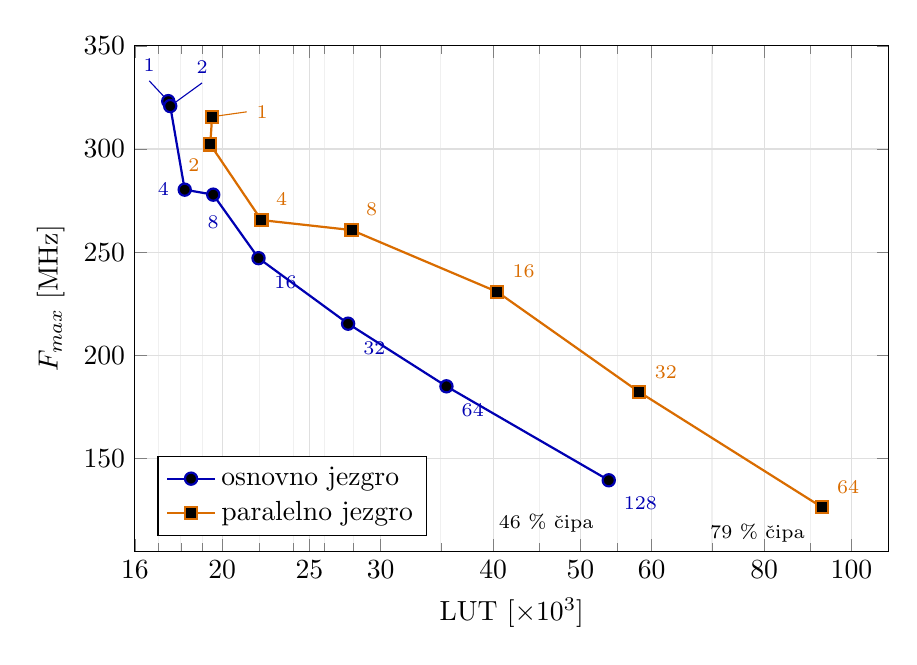
\begin{tikzpicture}
\begin{axis}[width=0.92\textwidth, height=8cm,
    xlabel={LUT [$\times 10^3$]}, ylabel={$F_{max}$ [MHz]},
    xmin=16, xmax=110, ymin=105, ymax=350, xmode=log, log basis x=10,
    xtick={16,20,25,30,40,50,60,80,100}, xticklabels={16,20,25,30,40,50,60,80,100},
    minor xtick={17,18,19,22,24,26,28,35,45,55,70,90},
    log ticks with fixed point,
    grid=both, major grid style={gray!25}, minor grid style={gray!12},
    legend pos=south west, legend cell align=left,
    every axis plot/.append style={thick, mark size=2.2pt}]
\addplot[mark=*, draw=blue!70!black]
    coordinates {(17.426,323.17) (17.515,320.79) (18.176,280.26) (19.551,277.84)
                 (21.951,247.05) (27.602,215.29) (35.497,184.93) (53.759,139.38)};
\addlegendentry{osnovno jezgro}
\addplot[mark=square*, draw=orange!85!black]
    coordinates {(19.495,315.62) (19.404,302.18) (22.109,265.52) (27.847,260.68)
                 (40.409,230.74) (58.112,182.15) (92.710,126.35)};
\addlegendentry{paralelno jezgro}
% Pri D = 1 i D = 2 tacke se po zauzecu gotovo poklapaju; plave oznake
% imaju izvodnicu, ostale stoje uz samu tacku.
\draw[blue!70!black, thin] (axis cs:17.426,323.17) -- (axis cs:16.6,333);
\node[font=\scriptsize, color=blue!70!black, anchor=south] at (axis cs:16.6,333) {1};
\draw[blue!70!black, thin] (axis cs:17.515,320.79) -- (axis cs:19.0,332);
\node[font=\scriptsize, color=blue!70!black, anchor=south] at (axis cs:19.0,332) {2};
\node[font=\scriptsize, color=blue!70!black, anchor=east]       at (axis cs:17.9,280.26) {4};
\node[font=\scriptsize, color=blue!70!black, anchor=north]      at (axis cs:19.551,272) {8};
\node[font=\scriptsize, color=blue!70!black, anchor=north west] at (axis cs:22.3,243) {16};
\node[font=\scriptsize, color=blue!70!black, anchor=north west] at (axis cs:28.0,211) {32};
\node[font=\scriptsize, color=blue!70!black, anchor=north west] at (axis cs:36.0,181) {64};
\node[font=\scriptsize, color=blue!70!black, anchor=north west] at (axis cs:54.5,136) {128};
\draw[orange!85!black, thin] (axis cs:19.495,315.62) -- (axis cs:21.3,318);
\node[font=\scriptsize, color=orange!85!black, anchor=west] at (axis cs:21.3,318) {1};
\node[font=\scriptsize, color=orange!85!black, anchor=north east] at (axis cs:19.35,300) {2};
\node[font=\scriptsize, color=orange!85!black, anchor=south west] at (axis cs:22.4,268) {4};
\node[font=\scriptsize, color=orange!85!black, anchor=south west] at (axis cs:28.2,263) {8};
\node[font=\scriptsize, color=orange!85!black, anchor=south west] at (axis cs:41.0,233) {16};
\node[font=\scriptsize, color=orange!85!black, anchor=south west] at (axis cs:59.0,184) {32};
\node[font=\scriptsize, color=orange!85!black, anchor=south west] at (axis cs:94.0,128) {64};
\node[font=\scriptsize, anchor=north east] at (axis cs:53.0,128) {46 \% čipa};
\node[font=\scriptsize, anchor=north east] at (axis cs:91.0,123) {79 \% čipa};
\end{axis}
\end{tikzpicture}
\caption{Zauzeće i radna učestanost ECDH jezgra po vrednostima generika \texttt{G\_D}. Uz tačku osnovnog jezgra sa $D = 128$ i paralelnog sa $D = 64$ označeno je i zauzeće u procentima čipa}
\label{fig:ecdh_pareto}
\end{figure}

Radna učestanost opada sa širinom obrade, ali znatno sporije nego što pada broj taktova množenja. Od $D = 1$ do $D = 128$ broj taktova po množenju padne 114 puta, sa 571 na 5, a učestanost osnovnog jezgra 2,3 puta, sa 323 na 139 MHz. Šira obrada zato množenje zaista skraćuje, čime je izmeren kompromis najavljen u odeljku \ref{subsec:hw_ecdh_mul}. Koja je konfiguracija najbolja zavisi od toga šta se meri. Po zauzeću i radnoj učestanosti to je $D = 1$, koji je istovremeno i najmanji i najbrži po taktu, sa $17\,426$ LUT-ova i 323,17 MHz. Po vremenu jednog skalarnog množenja on je najslabiji. Već susedna tačka $D = 2$ po ta dva merila granično je lošija, 89 LUT-ova i $2{,}4$ MHz, a trajanje skraćuje 1,94 puta, gotovo dvostruko.
\smallbreak
Kritičnu putanju ne čini logika nego povezivanje. Kod osnovnog jezgra sa $D = 1$ logika troši $0{,}95$ ns, a veze $2{,}42$ ns, dakle 72 procenta putanje, i to pri zauzeću ispod petnaest procenata čipa. Radna učestanost jezgra nad poljem B-571 zato se ne može projektovati iz dubine logike, po čemu se ovo jezgro razlikuje od SHA-3 i AES-GCM akceleratora, koji zauzimaju po nekoliko procenata čipa, pa se zagušenje kod njih i ne javlja.

\begin{figure}[H]
\centering
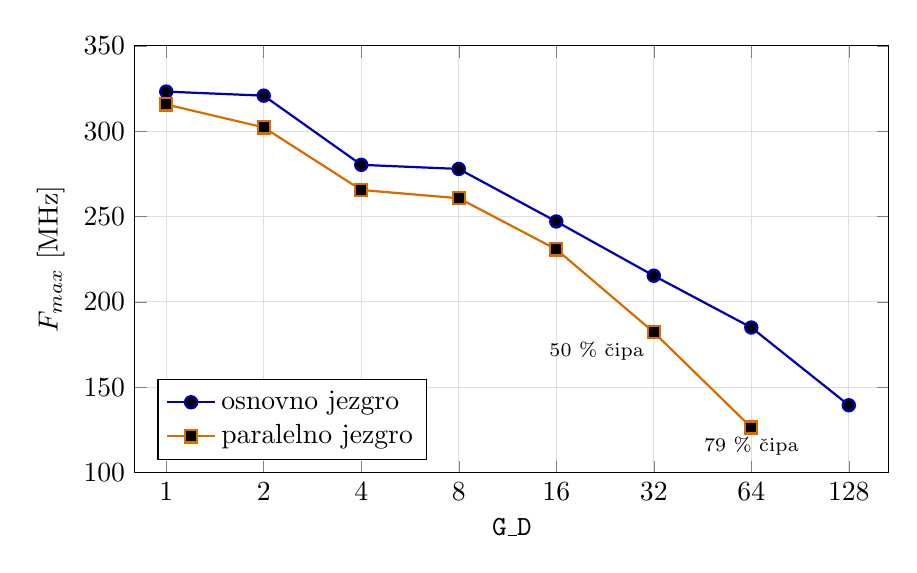
\begin{tikzpicture}
\begin{axis}[width=0.92\textwidth, height=7cm,
    xmode=log, log basis x=2,
    xtick={1,2,4,8,16,32,64,128}, xticklabels={1,2,4,8,16,32,64,128},
    xlabel={\texttt{G\_D}}, ylabel={$F_{max}$ [MHz]},
    xmin=0.8, xmax=170, ymin=100, ymax=350,
    grid=major, grid style={gray!25},
    legend pos=south west, legend cell align=left,
    every axis plot/.append style={thick, mark size=2.2pt}]
\addplot[mark=*, draw=blue!70!black] coordinates
    {(1,323.17) (2,320.79) (4,280.26) (8,277.84) (16,247.05) (32,215.29) (64,184.93) (128,139.38)};
\addlegendentry{osnovno jezgro}
\addplot[mark=square*, draw=orange!85!black] coordinates
    {(1,315.62) (2,302.18) (4,265.52) (8,260.68) (16,230.74) (32,182.15) (64,126.35)};
\addlegendentry{paralelno jezgro}
\node at (axis cs:32,182.15) [below left, font=\scriptsize] {50 \% čipa};
\node at (axis cs:64,126.35) [below, font=\scriptsize] {79 \% čipa};
\end{axis}
\end{tikzpicture}
\caption{Radna učestanost po vrednostima generika \texttt{G\_D}, sa zauzećem čipa uz dve tačke paralelnog jezgra}
\label{fig:ecdh_fmax_d}
\end{figure}

Gornju granicu mreže ne postavljaju vremenski uslovi nego kapacitet ploče. Paralelno jezgro sa $D = 128$ posle optimizacije traži $162\,863$ LUT-a, a čip ih ima $117\,120$, pa raspoređivanje odbija da počne i ta tačka u tabeli ne postoji. Uticaj zauzeća vidi se i pre same granice, na slici \ref{fig:ecdh_fmax_d}, poređenjem dva jezgra pri istoj širini obrade. Množač i njegov kombinacioni lanac su im isti, pa razlika u učestanosti pri istom $D$ potiče od gustine na čipu. Do $D = 16$ paralelno jezgro zaostaje za osnovnim najviše sedam procenata. Pri $D = 32$, gde zauzima polovinu čipa, zaostatak je petnaest procenata, a pri $D = 64$, na četiri petine čipa, trideset dva procenta. Raspoređivanju tada ponestaje prostora i zagušenje veza postaje glavno ograničenje, ispred dužine samog lanca. Jači čip bi te dve pojave razdvojio, jer bi isti dizajn na njemu zauzimao manji udeo površine, pa bi se video čist uticaj širine obrade.
\smallbreak
\subsection{Latencija skalarnog množenja}
\label{subsec:rez_ecdh_latencija}

Zauzeće i radna učestanost mere cenu jezgra, a ovaj odeljak meri šta se za tu cenu dobija. Koliko jedno skalarno množenje traje utvrđeno je takt-tačno u simulaciji, brojanjem ivica takta od one na kojoj jezgro prihvati zahtev do one na kojoj se pojavi znak kraja. Izlaz svakog prolaza poredi se sa afinim koordinatama iz referentnog modela, pa u tabelu ulazi samo trajanje uz koje je rezultat tačan. Merene su sve konfiguracije iz tabela \ref{tab:ecdh_impl_f1} i \ref{tab:ecdh_impl_f2}, kao i broj taktova paralelnog jezgra sa $D = 128$, uz istu vrednost skalara, čija najviša jedinica stoji na 570. mestu, na najdužoj poziciji koju standardni ključ dopušta, pa poravnanje skalara u svakom redu košta isto.
\smallbreak
Meri se samo jezgro, bez AXI4-Stream omotača, jer omotač na portove ne izvodi signal kojim jezgro označava kraj računa. Obim se time razlikuje od prethodnog odeljka, gde je merena površina celog IP-a. Razlika je poznata i mala. Omotač po jednom pozivu jezgra prenese komandnu reč i četiri koordinate, dve ulazne i dve izlazne, po devet reči na magistrali od 64 bita, dakle trideset sedam taktova, što je ispod pola procenta i najkraćeg trajanja u tabeli.

\begin{table}[H]
\caption{Trajanje jednog skalarnog množenja. Kolona $q = \lceil 571/D \rceil$ je broj digita koje množač obradi po jednom množenju u polju. Vreme $t$ dobija se deljenjem broja taktova radnom učestanošću iz tabela \ref{tab:ecdh_impl_f1} i \ref{tab:ecdh_impl_f2}, a poslednja kolona je odnos broja taktova dva jezgra pri istom $D$. Paralelno jezgro sa $D = 128$ nema vreme jer ne staje na ploču, pa mu se broj taktova zna iz simulacije, a radna učestanost ne postoji}
\centering
{\renewcommand{\arraystretch}{1.25}
\resizebox{0.86\textwidth}{!}{
\begin{tabular}{|c|c|c|c|c|c|c|}
\hline
\rowcolor{gray!30}
\multicolumn{2}{|c|}{} & \multicolumn{2}{c|}{osnovno jezgro} & \multicolumn{2}{c|}{paralelno jezgro} & \\
\cline{3-6}
\rowcolor{gray!30}
\texttt{G\_D} & $q$ & taktova & $t$ [$\mu$s] & taktova & $t$ [$\mu$s] & \multirow{-2}{*}{odnos taktova} \\
\hline
1   & 571 & 2\,005\,406 & 6205,4 & 670\,468 & 2124,3 & 2,99 \\
\hline
2   & 286 & 1\,023\,866 & 3191,7 & 338\,728 & 1120,9 & 3,02 \\
\hline
4   & 143 & 531\,374 & 1896,0 & 172\,276 & 648,8 & 3,08 \\
\hline
8   & 72  & 286\,850 & 1032,4 & 89\,632 & 343,8 & 3,20 \\
\hline
16  & 36  & 162\,866 & 659,2  & 47\,728 & 206,8 & 3,41 \\
\hline
32  & 18  & 100\,874 & 468,5  & 26\,776 & 147,0 & 3,77 \\
\hline
64  & 9   & 69\,878  & 377,9  & 16\,300 & 129,0 & 4,29 \\
\hline
128 & 5   & 56\,102  & 402,5  & 11\,644 & --- & 4,82 \\
\hline
\end{tabular}
}}
\label{tab:ecdh_latencija}
\end{table}

Broj taktova po iteraciji merdevina linearan je u $q$, a prave kroz izmerene tačke glase
\begin{align}
    T^{\mathrm{I}}_{\mathrm{iter}}  &= 6{,}04 \cdot q + 68, \label{eq:ecdh_iter_f1} \\
    T^{\mathrm{II}}_{\mathrm{iter}} &= 2{,}04 \cdot q + 10, \label{eq:ecdh_iter_f2}
\end{align}
Nagibi su šest i dva, čime je procena iz odeljka \ref{subsec:hw_ecdh_korak} potvrđena na obe realizacije. Slobodni član je ono što ta procena ne obuhvata. Osnovno jezgro troši šezdeset osam taktova po iteraciji na kvadriranja, sabiranja i pozive aritmetičke jedinice po svakoj od četrnaest operacija, a paralelno deset, jer kod njega kvadriranja i sabiranja teku u prolazu između dve runde množenja.

Time je objašnjeno i kretanje odnosa u poslednjoj koloni tabele \ref{tab:ecdh_latencija}. Pri $D = 1$ odnos iznosi $2{,}99$, dakle upravo šest prema dva, jer je $q$ toliko veliko da množenja odrede celu cenu. Sa porastom $D$ broj digita opada, udeo slobodnog člana raste, a kako je on kod osnovnog jezgra skoro sedam puta veći, odnos se penje do $4{,}82$ pri $D = 128$. Prednost paralelnog jezgra utoliko je veća ukoliko je obrada šira.

Izmereno trajanje popunjava i analitičku procenu iz odeljka \ref{subsec:montgomery}. Ukupan broj taktova prati $T^{\mathrm{I}} = 3444 \cdot q + 38\,882$ za osnovno i $T^{\mathrm{II}} = 1164 \cdot q + 5824$ za paralelno jezgro, i oba izraza pogađaju svih šesnaest redova tabele bez ostatka. Nagib osnovnog jezgra tačno je broj množenja u polju, a razlika nagiba, $2280 = 570 \cdot 4$, dolazi otud što šest množenja iteracije na tri množača staju u vreme dva, pa svaka od 570 iteracija uštedi vreme četiri množenja. Slobodni član obuhvata i režiju iteracija i celu završnu konverziju sa jednom inverzijom. Pri $D = 64$ množenja tako nose $3444 \cdot 9 = 30\,996$ taktova, režija preostalih $38\,882$, a zbir je upravo izmerenih $69\,878$. Na 184,93 MHz to je $377{,}9$ mikrosekundi po skalarnom množenju, dok paralelno jezgro pri istoj širini traži $129{,}0$. Najbrža konfiguracija time opsluži oko 3875 razmena ključa u sekundi, jer 129,0 mikrosekundi daje 7751 množenje u sekundi, a razmena traži dva poziva jezgra.

Uz cenu iz tabela zauzeća sada se može reći koja konfiguracija najbolje troši površinu. Proizvod broja LUT-ova i trajanja najmanji je za paralelno jezgro sa $D = 16$, gde iznosi $8{,}4$ miliona LUT-mikrosekundi, s tim što je susedna tačka $D = 32$ na $8{,}5$ miliona, unutar šuma alata, pa je radna tačka paralelnog jezgra ceo opseg od 16 do 32. Najbolja vrednost osnovnog jezgra je $12{,}9$ miliona pri $D = 32$, pa je paralelno jezgro trećinu povoljnije. Poređenje na bliskoj površini je neposrednije. Paralelno jezgro sa $D = 32$ zauzima $58\,112$ LUT-ova i završi za $147{,}0$ mikrosekundi, a osnovno sa $D = 128$ zauzima $53\,759$ LUT-ova i završi za $402{,}5$ mikrosekundi, pa za osam procenata više logike daje $2{,}7$ puta kraće trajanje.

Ceo kompromis prikazan je na slici \ref{fig:ecdh_cena_korist}, gde svakoj konfiguraciji odgovara jedna tačka sa zauzećem na jednoj i trajanjem na drugoj osi. Povoljne konfiguracije leže bliže donjem levom uglu, jer troše manje i logike i vremena.

\begin{figure}[H]
\centering
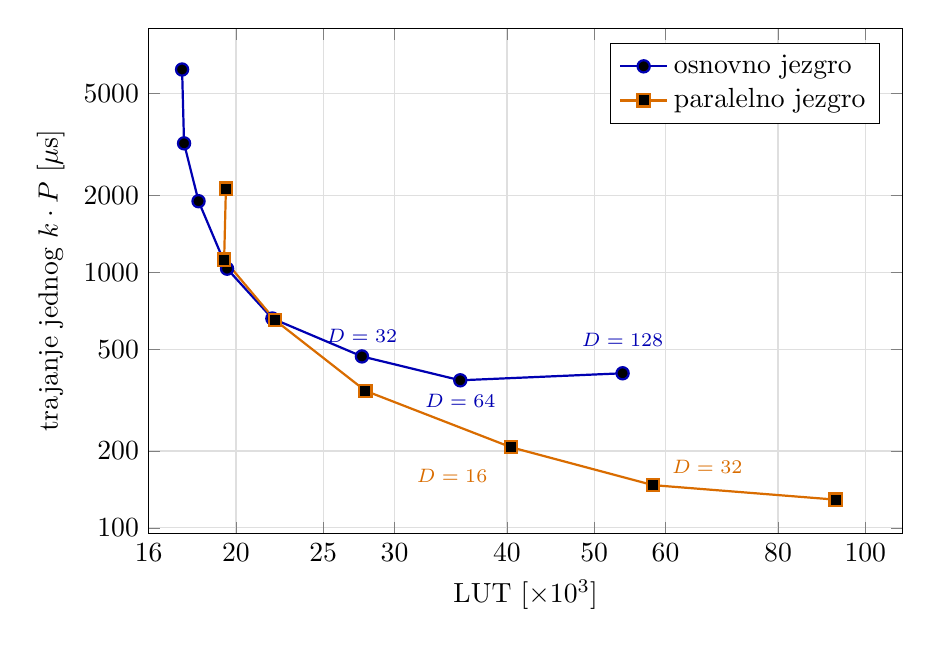
\begin{tikzpicture}
\begin{axis}[width=0.92\textwidth, height=8cm,
    xlabel={LUT [$\times 10^3$]}, ylabel={trajanje jednog $k \cdot P$ [$\mu$s]},
    xmin=16, xmax=110, ymin=95, ymax=9000,
    xmode=log, log basis x=10, ymode=log, log basis y=10,
    xtick={16,20,25,30,40,50,60,80,100}, xticklabels={16,20,25,30,40,50,60,80,100},
    ytick={100,200,500,1000,2000,5000}, yticklabels={100,200,500,1000,2000,5000},
    log ticks with fixed point,
    grid=major, grid style={gray!25},
    legend pos=north east, legend cell align=left,
    every axis plot/.append style={thick, mark size=2.2pt}]
\addplot[mark=*, draw=blue!70!black]
    coordinates {(17.426,6205.4) (17.515,3191.7) (18.176,1896.0) (19.551,1032.4)
                 (21.951,659.2) (27.602,468.5) (35.497,377.9) (53.759,402.5)};
\addlegendentry{osnovno jezgro}
\addplot[mark=square*, draw=orange!85!black]
    coordinates {(19.495,2124.3) (19.404,1120.9) (22.109,648.8) (27.847,343.8)
                 (40.409,206.8) (58.112,147.0) (92.710,129.0)};
\addlegendentry{paralelno jezgro}
\node[font=\scriptsize, color=blue!70!black, anchor=south]        at (axis cs:27.602,485) {$D = 32$};
\node[font=\scriptsize, color=blue!70!black, anchor=north]        at (axis cs:35.497,365) {$D = 64$};
\node[font=\scriptsize, color=blue!70!black, anchor=south]        at (axis cs:53.759,470) {$D = 128$};
\node[font=\scriptsize, color=orange!85!black, anchor=north east] at (axis cs:39.0,186) {$D = 16$};
\node[font=\scriptsize, color=orange!85!black, anchor=south west] at (axis cs:59.5,150) {$D = 32$};
\end{axis}
\end{tikzpicture}
\caption{Zauzeće i trajanje jednog skalarnog množenja za sve merene konfiguracije. Označeno je pet tačaka o kojima govori tekst}
\label{fig:ecdh_cena_korist}
\end{figure}

Kod osnovnog jezgra širina obrade ima i granicu koja nije kapacitet ploče. Pri $D = 128$ ono traje $402{,}5$ mikrosekundi, dakle duže nego pri $D = 64$ sa $377{,}9$, a traži pedeset jedan procenat više LUT-ova, jer pad učestanosti sa $184{,}93$ na $139{,}38$ MHz nadjača uštedu u taktovima. Poslednji korak udvostručenja širine tu se ne isplati. Kod paralelnog jezgra poslednji korak koji staje na ploču, sa $D = 32$ na 64, još se isplati, jer trajanje opada sa $147{,}0$ na $129{,}0$ mikrosekundi.

\section{SHA-3 akcelerator}
\label{sec:rez_sha3}

\subsection{Provera po nivoima}
\label{subsec:rez_sha3_provera}

Ispravnost je proverena testovima sa poznatim odgovorima nad celim IP-om, za sve četiri SHA3 varijante, obe SHAKE funkcije i cSHAKE, u kombinacijama širine magistrale od 8 do 64 bita, sa jednom ili dve runde po taktu, a kod varijante SHA3-256 sa svih osam delilaca broja 24. Vektore proizvodi referentni model iz odeljka \ref{sec:rez_metodologija}, nad porukama uzastopnih dužina, od jednog bajta do višeblokovnih, pa dopuna prođe kroz svaki položaj u reči i preko granice bloka. Softversko uokvirivanje KMAC funkcije provereno je nad KMAC256 i KMACXOF256 vektorima, čime je pokrivena podela posla iz odeljka \ref{subsec:hw_sha3_kmac}, po kojoj uokvirivanje pripada strani koja podatke dovodi.
\smallbreak
Namenski testovi gustog saobraćaja uz to drže ulaz spremnim u svakom taktu, šalju pakete bez razmaka i koče izlaz nasumičnim protivpritiskom, pa obuhvataju granične slučajeve upravljanja tokom, među njima i upis dopune u već pun blok, dok je \texttt{tready} spušten (odeljak \ref{subsec:hw_sha3_ib}). Jezgro je provereno i na ploči, gde se sažeci porede sa vrednostima OpenSSL biblioteke.

\subsection{Zauzeće resursa i radna učestanost}
\label{subsec:rez_sha3_resursi}

Obe arhitekture iz odeljka \ref{subsec:hw_sha3_dve} implementirane su za sve četiri varijante standarda i obe širine magistrale za koje je merena i propusnost, 32 i 64 bita, ukupno četrnaest konfiguracija. Širine od 8 i 16 bita su izostavljene, jer su ulazno ograničene u svim varijantama, pa za poređenje arhitektura ne donose ništa novo. Kombinacija SHA3-224 sa magistralom od 64 bita ne postoji, jer sažetak od 224 bita nije deljiv širinom magistrale, pa se ta kombinacija odbacuje još pri elaboraciji. Rezultati su dati u tabelama \ref{tab:sha3_impl_a1} i \ref{tab:sha3_impl_a2}.

\begin{table}[H]
\caption{Arhitektura I (jedna runda po taktu), implementacija van konteksta. Kolona usko grlo sledi iz modela u odeljku \ref{subsec:rez_sha3_propusnost}}
\centering
{\renewcommand{\arraystretch}{1.25}
\resizebox{0.80\textwidth}{!}{
\begin{tabular}{|c|c|c|c|c|c|}
\hline
\rowcolor{gray!30}
Varijanta & \texttt{DATA\_WIDTH} & LUT & FF & $F_{max}$ [MHz] & usko grlo \\
\hline
SHA3-224                  & 32 & 5369 & 3090 & 418,76 & ulaz \\
\hline
\multirow{2}{*}{SHA3-256} & 32 & 5331 & 3070 & 412,54 & ulaz \\
                          & 64 & 5591 & 3130 & 432,90 & permutacija \\
\hline
\multirow{2}{*}{SHA3-384} & 32 & 5136 & 2933 & 442,28 & ulaz \\
                          & 64 & 5472 & 3004 & 424,27 & permutacija \\
\hline
\multirow{2}{*}{SHA3-512} & 32 & 4537 & 2807 & 430,11 & permutacija \\
                          & 64 & 4803 & 2882 & 424,99 & permutacija \\
\hline
\end{tabular}
}}
\label{tab:sha3_impl_a1}
\end{table}

\begin{table}[H]
\caption{Arhitektura II (dve runde po taktu), implementacija van konteksta. Kolona usko grlo sledi iz modela u odeljku \ref{subsec:rez_sha3_propusnost}}
\centering
{\renewcommand{\arraystretch}{1.25}
\resizebox{0.80\textwidth}{!}{
\begin{tabular}{|c|c|c|c|c|c|}
\hline
\rowcolor{gray!30}
Varijanta & \texttt{DATA\_WIDTH} & LUT & FF & $F_{max}$ [MHz] & usko grlo \\
\hline
SHA3-224                  & 32 & 10107 & 3085 & 235,85 & ulaz \\
\hline
\multirow{2}{*}{SHA3-256} & 32 & 10579 & 3070 & 228,73 & ulaz \\
                          & 64 & 10137 & 3128 & 241,66 & ulaz \\
\hline
\multirow{2}{*}{SHA3-384} & 32 & 9496 & 2927 & 242,37 & ulaz \\
                          & 64 & 10023 & 3009 & 253,23 & ulaz \\
\hline
\multirow{2}{*}{SHA3-512} & 32 & 9163 & 2800 & 233,10 & ulaz \\
                          & 64 & 9479 & 2876 & 234,58 & permutacija \\
\hline
\end{tabular}
}}
\label{tab:sha3_impl_a2}
\end{table}

Odnos dve arhitekture isti je u svih sedam parova. Arhitektura I postiže preko 400 MHz u svih sedam konfiguracija, a druga plaća od 40 do 46 procenata radne učestanosti, a njena cena u logici iznosi od 1,81 do 2,02 puta više LUT-ova, dakle blizu dvostruke površine. Broj flipflopova se pritom praktično ne menja, jer obe arhitekture drže isto stanje od 1600 bitova, pa je cena u logici, a ne u registrima. Manji $rate$ znači uži ulazni bafer, pa SHA3-512 troši najmanje logike u obe arhitekture. Raspored svih četrnaest tačaka prikazan je na slici \ref{fig:sha3_lut_fmax}.

\begin{figure}[H]
\centering
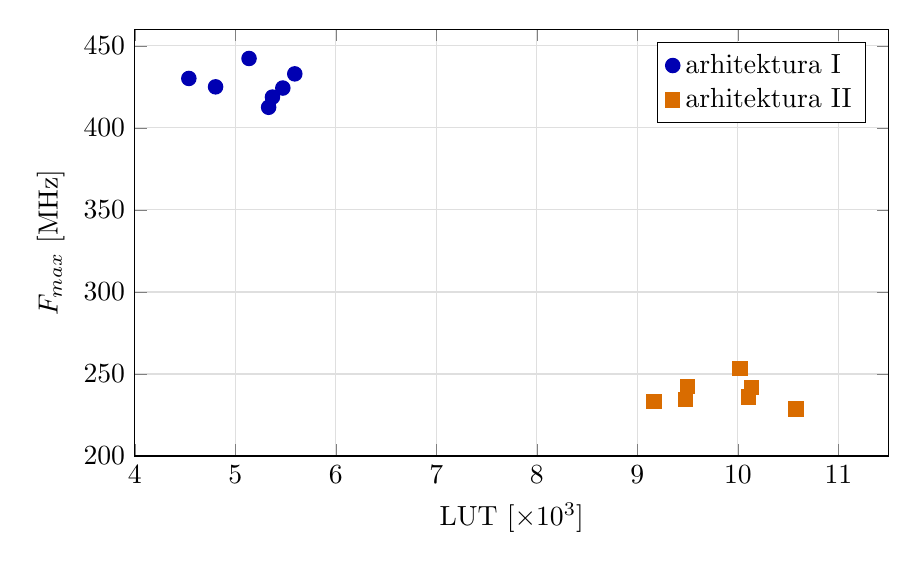
\begin{tikzpicture}
\begin{axis}[width=0.92\textwidth, height=7cm,
    xlabel={LUT [$\times 10^3$]}, ylabel={$F_{max}$ [MHz]},
    xmin=4, xmax=11.5, ymin=200, ymax=460,
    grid=major, grid style={gray!25},
    legend pos=north east, legend cell align=left,
    every axis plot/.append style={only marks, mark size=2.6pt}]
\addplot[mark=*, draw=blue!70!black, fill=blue!70!black] coordinates
    {(5.369,418.76) (5.331,412.54) (5.591,432.90) (5.136,442.28) (5.472,424.27) (4.537,430.11) (4.803,424.99)};
\addlegendentry{arhitektura I}
\addplot[mark=square*, draw=orange!85!black, fill=orange!85!black] coordinates
    {(10.107,235.85) (10.579,228.73) (10.137,241.66) (9.496,242.37) (10.023,253.23) (9.163,233.10) (9.479,234.58)};
\addlegendentry{arhitektura II}
\end{axis}
\end{tikzpicture}
\caption{Zauzeće i radna učestanost svih četrnaest SHA-3 konfiguracija}
\label{fig:sha3_lut_fmax}
\end{figure}

\subsection{Propusnost i model uskog grla}
\label{subsec:rez_sha3_propusnost}

Propusnost je izmerena takt-tačno u simulaciji, nad porukom od pedeset blokova, uz ulaz spreman u svakom taktu i izlaz prihvatan bez zastoja. Rezultati su dati u tabeli \ref{tab:sha3_bpc}.

\begin{table}[H]
\caption{Izmerena vrednost bita po taktu i propusnost izvedena iz nje pri $F_{max}$ iz tabela \ref{tab:sha3_impl_a1} i \ref{tab:sha3_impl_a2}}
\centering
\resizebox{\textwidth}{!}{
\begin{tabular}{|c|c|c|c|c|c|}
\hline
\rowcolor{gray!30}
Konfiguracija & \texttt{DATA\_WIDTH} & Arhitektura & Bita po taktu & Propusnost [Gb/s] & Usko grlo \\
\hline
SHA3-256 & 32 & I  & 30,49 & 12,58 & ulaz \\
\hline
SHA3-256 & 32 & II & 30,69 & 7,02 & ulaz \\
\hline
SHA3-256 & 64 & I  & 42,71 & 18,49 & permutacija \\
\hline
SHA3-256 & 64 & II & 59,25 & 14,32 & ulaz \\
\hline
SHA3-512 & 32 & I  & 22,38 & 9,63 & permutacija \\
\hline
SHA3-512 & 32 & II & 29,38 & 6,85 & ulaz \\
\hline
SHA3-512 & 64 & I  & 22,66 & 9,63 & permutacija \\
\hline
SHA3-512 & 64 & II & 43,01 & 10,09 & permutacija \\
\hline
\end{tabular}
}
\label{tab:sha3_bpc}
\end{table}

Ponašanje se u celini objašnjava jednostavnim modelom. Po bloku od $rate$ bitova troši se
\begin{equation}
    T_{blok} = \max\!\left(\frac{rate}{\texttt{DATA\_WIDTH}},\; \frac{24}{\texttt{ROUNDS\_PER\_CYCLE}}\right) + 1 \ \text{takt},
    \label{eq:sha3_model}
\end{equation}
gde prvi član broji reči potrebne da se blok unese, a drugi trajanje permutacije. Maksimum stoji zato što se punjenje narednog bloka i permutacija tekućeg preklapaju, kako je opisano u odeljku \ref{subsec:hw_sha3_arh}, pa brzinu određuje sporiji od njih. Sama pretpostavka o preklapanju proverena je zasebnim testom sa brojačima taktova, koji potvrđuje da se reči primaju tokom permutacije, da se naredni isceđeni deo permutuje dok se prethodni iznosi i da reči naredne poruke ulaze dok izlaz prethodne još teče, a sažeci se pritom i dalje poklapaju sa referentnim.

Dodatni takt je predaja bloka i plaća se na obe strane, zbog čega i stoji izvan maksimuma. Kada je usko grlo unos, ulazni bafer posle poslednje reči spušta \texttt{tready} i u tom taktu predaje popunjen blok jezgru umesto da prima novu reč, po odeljku \ref{subsec:hw_sha3_ib}. Kada je usko grlo permutacija, jezgro posle dvadeset četvrte runde ne ulazi pravo u narednu, nego jedan takt čeka blok. Kod SHA3-256 sa magistralom od 32 bita to je $34 + 1 = 35$ taktova, a kod iste varijante sa magistralom od 64 bita, gde permutacija preuzima ulogu uskog grla, $24 + 1 = 25$. Primenjen na svih četrnaest konfiguracija, model ulaz proglašava uskim grlom u devet, a permutaciju u pet, kako je upisano u tabelama \ref{tab:sha3_impl_a1} i \ref{tab:sha3_impl_a2}.

Izmerene vrednosti uz cenu po bloku nose i završnu permutaciju sa ispisom sažetka, između sedamnaest i trideset pet taktova, koja se plaća jednom po poruci. Kada se i ona uračuna, model daje izmereni broj taktova tačno, pa je za SHA3-256 sa magistralom od 32 bita u prvoj arhitekturi $50 \cdot 35 + 33 = 1783$ takta, koliko je i izmereno. Kolona bita po taktu potiče iz istog merenja, a od količnika $rate$ i cene bloka razlikuje se zato što je merna poruka za jednu reč kraća od pedeset punih blokova, da bi dopuna ostala unutar poslednjeg bloka. Sa dužinom poruke udeo završnog repa opada, pa propusnost teži vrednosti od jedan do tri procenta višoj od navedene u tabeli \ref{tab:sha3_bpc}.
\smallbreak
Iz modela sledi i pravilo za izbor arhitekture, strože nego što se na prvi pogled čini. Druga arhitektura prepolovljuje broj taktova permutacije, ali ne i vreme, jer sa dužom kritičnom putanjom radna učestanost pada od 40 do 46 procenata. Da bi ukupna propusnost porasla, dobitak u bitima po taktu mora da nadmaši taj gubitak, dakle da bude veći od približno 1,8 puta, a njega uopšte nema tamo gde granicu postavlja ulaz. Kod SHA3-256 sa magistralom od 32 bita cena bloka ostaje 35 taktova u obe arhitekture, pa druga gubi celih 44 procenta propusnosti. Kod SHA3-256 sa 64 bita i SHA3-512 sa 32 bita permutacija jeste usko grlo prve arhitekture, ali skraćenje donosi svega 1,4 odnosno 1,3 puta, pa druga ostaje 23 odnosno 29 procenata ispod prve. Prag prelazi jedino SHA3-512 sa 64 bita, gde dobitak u bitima po taktu iznosi 1,9 puta, po modelu 25 naspram 13 taktova po bloku, pa je druga arhitektura ispred, 10,09 naspram 9,63 Gb/s, za nepunih pet procenata, razliku unutar šuma alata, i po ceni dvostruke logike. Za SHA3-224, čija propusnost nije merena, isti zaključak daje sam model. Tamo je $rate$ najveći ($1152$ bita), pa unos bloka traje duže od permutacije, njeno skraćivanje ne menja ništa, a niža učestanost ostaje čist gubitak. Odnosi za sve četiri merene kombinacije prikazani su na slici \ref{fig:sha3_gbps}.

\begin{figure}[H]
\centering
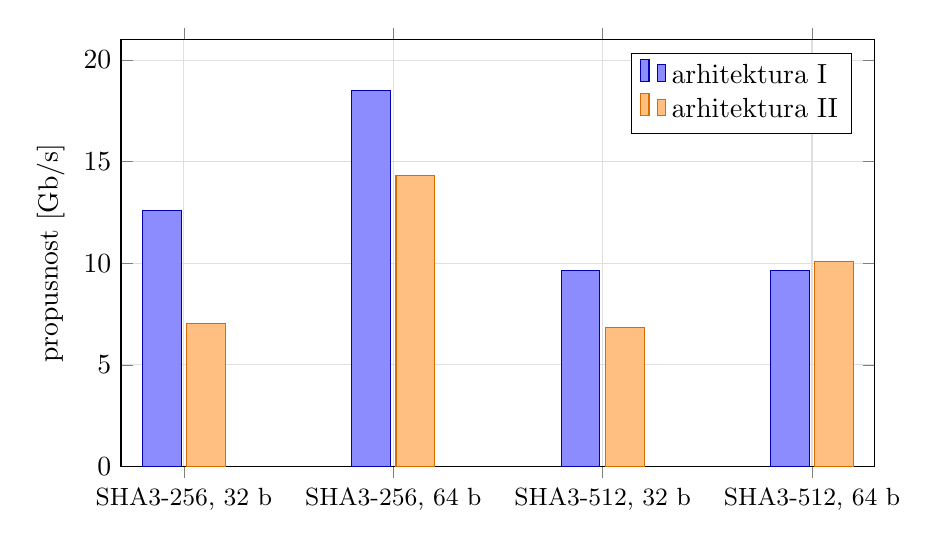
\begin{tikzpicture}
\begin{axis}[width=0.92\textwidth, height=7cm, ybar, bar width=14pt,
    ylabel={propusnost [Gb/s]}, ymin=0, ymax=21,
    symbolic x coords={{SHA3-256, 32 b},{SHA3-256, 64 b},{SHA3-512, 32 b},{SHA3-512, 64 b}},
    xtick=data, x tick label style={font=\small},
    grid=major, grid style={gray!25},
    legend pos=north east, legend cell align=left]
\addplot[draw=blue!70!black, fill=blue!45] coordinates
    {({SHA3-256, 32 b},12.58) ({SHA3-256, 64 b},18.49) ({SHA3-512, 32 b},9.63) ({SHA3-512, 64 b},9.63)};
\addlegendentry{arhitektura I}
\addplot[draw=orange!85!black, fill=orange!50] coordinates
    {({SHA3-256, 32 b},7.02) ({SHA3-256, 64 b},14.32) ({SHA3-512, 32 b},6.85) ({SHA3-512, 64 b},10.09)};
\addlegendentry{arhitektura II}
\end{axis}
\end{tikzpicture}
\caption{Propusnost dve arhitekture za četiri merene kombinacije varijante i širine magistrale, pri izmerenoj radnoj učestanosti}
\label{fig:sha3_gbps}
\end{figure}

Za kratke poruke merodavna je latencija, a ne propusnost. Za poruku od šesnaest bajtova ona iznosi 39 taktova kod SHA3-256 pri širini od 32 bita u prvoj arhitekturi, odnosno 21 takt pri širini od 64 bita u drugoj. U profilu koji odgovara izvođenju ključeva KMAC okvir iz odeljka \ref{subsec:kmac} nosi tri bloka, prefiksni, blok ključa i blok sa tajnom $Z$, a ključ od 256 bitova staje u prvo ceđenje. Izvođenje ključa zato staje u tri cene bloka iz jednačine \eqref{eq:sha3_model} uz rep poruke, $3 \cdot 18 + 17 = 71$ takt pri širini od 64 bita u drugoj arhitekturi, a najviše $3 \cdot 35 + 33 = 138$ taktova u prvoj pri 32 bita, jer treći blok nije pun. Na izmerenim učestanostima to je oko tri desetinke mikrosekunde, zanemarljivo u odnosu na trajanje razmene ključeva, pa izbor konfiguracije za tu ulogu nije kritičan. Određuje ga AES-GCM strana sistema.

\subsection{Upravljački program i merni put}
\label{subsec:rez_sha3_drajver}

Merenja na ploči obuhvataju ceo put od datoteke do sažetka, pa ono što se meri nije samo jezgro nego i softver oko njega. Za potrebe ovog rada napisan je upravljački program jezgra operativnog sistema (engl. \textit{kernel module}) za PetaLinux, zajedno sa dva korisnička programa koji ga koriste, jer se bez tog sloja jezgro sa procesorske strane ne može pokrenuti.
\smallbreak
Program se sa jezgrom povezuje preko opisa uređaja u stablu uređaja (engl. \textit{device tree}) i korisniku nudi dve datoteke uređaja (engl. \textit{character device}), jednu za slanje poruke i jednu za prijem sažetka. Prenos vodi kroz podsistem \texttt{DMA Engine} jezgra operativnog sistema, a ne programiranjem registara kontrolera. Put podataka u tim merenjima prikazan je na slici \ref{fig:sha3_dma_put}.

\begin{figure}[H]
\centering
\resizebox{\textwidth}{!}{
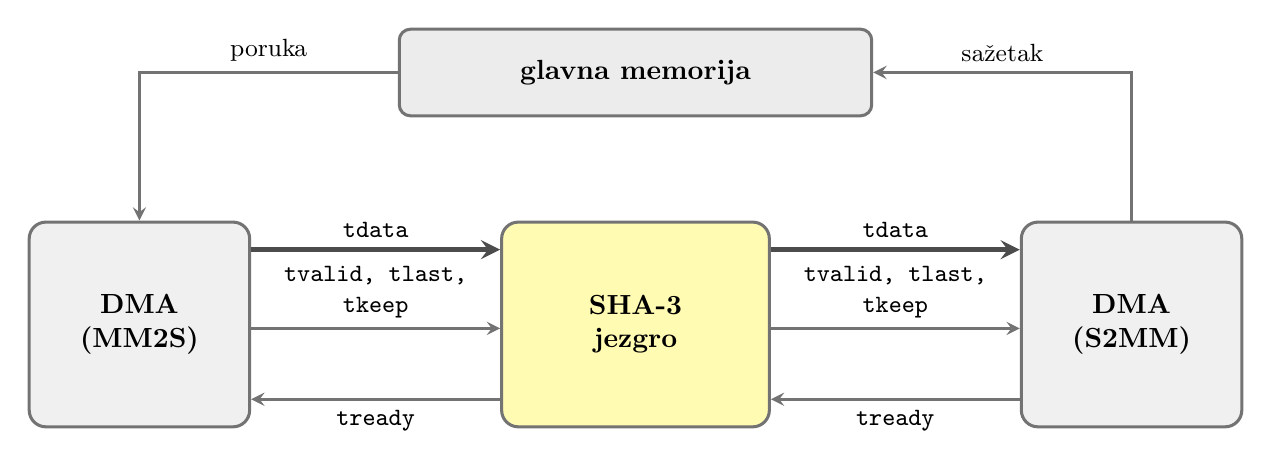
\begin{tikzpicture}[>=stealth]
    \node (mem)  [draw=black!55, line width=1.1pt, fill=gray!15, rounded corners=4pt, minimum width=6.0cm, minimum height=1.1cm, font=\bfseries] at (7.5,3.2) {glavna memorija};
    \node (dma1) [draw=black!55, line width=1.1pt, fill=gray!12, rounded corners=6pt, minimum width=2.8cm, minimum height=2.6cm, font=\bfseries, align=center] at (1.2,0) {DMA\\ (MM2S)};
    \node (acc)  [draw=black!55, line width=1.1pt, fill=yellow!30, rounded corners=6pt, minimum width=3.4cm, minimum height=2.6cm, font=\bfseries, align=center] at (7.5,0) {SHA-3\\ jezgro};
    \node (dma2) [draw=black!55, line width=1.1pt, fill=gray!12, rounded corners=6pt, minimum width=2.8cm, minimum height=2.6cm, font=\bfseries, align=center] at (13.8,0) {DMA\\ (S2MM)};
    % memorija -> MM2S i S2MM -> memorija
    \draw [draw=black!55, line width=1.1pt, ->]
        (mem.west) -- node[above, font=\small] {poruka} (1.2,3.2) -- (dma1.north);
    \draw [draw=black!55, line width=1.1pt, ->]
        (dma2.north) -- (13.8,3.2) -- node[above, font=\small] {sažetak} (mem.east);
    % ulazni signali (DMA -> jezgro)
    \draw [draw=black!70, line width=2pt, ->]
        ([yshift=0.95cm]dma1.east) -- node[above, font=\small\ttfamily] {tdata} ([yshift=0.95cm]acc.west);
    \draw [draw=black!55, line width=1.1pt, ->]
        ([yshift=-0.05cm]dma1.east) -- node[above, font=\small\ttfamily, align=center] {tvalid, tlast,\\ tkeep} ([yshift=-0.05cm]acc.west);
    \draw [draw=black!55, line width=1.1pt, ->]
        ([yshift=-0.95cm]acc.west) -- node[below, font=\small\ttfamily] {tready} ([yshift=-0.95cm]dma1.east);
    % izlazni signali (jezgro -> DMA)
    \draw [draw=black!70, line width=2pt, ->]
        ([yshift=0.95cm]acc.east) -- node[above, font=\small\ttfamily] {tdata} ([yshift=0.95cm]dma2.west);
    \draw [draw=black!55, line width=1.1pt, ->]
        ([yshift=-0.05cm]acc.east) -- node[above, font=\small\ttfamily, align=center] {tvalid, tlast,\\ tkeep} ([yshift=-0.05cm]dma2.west);
    \draw [draw=black!55, line width=1.1pt, ->]
        ([yshift=-0.95cm]dma2.west) -- node[below, font=\small\ttfamily] {tready} ([yshift=-0.95cm]acc.east);
\end{tikzpicture}
}
\caption[Put podataka u merenjima na ploči]{Put podataka u merenjima na ploči: kanal MM2S čita poruku iz glavne memorije i pretvara je u AXI4-Stream tok, a kanal S2MM sažetak vraća u memoriju. Procesor u samom prenosu ne učestvuje}
\label{fig:sha3_dma_put}
\end{figure}

Tri svojstva tog puta određuju izmerene brojeve.
\begin{itemize}[itemsep=2pt]
    \item Cela datoteka prenosi se u jednom DMA prenosu, jer granicu poruke označava signal \texttt{tlast}, na kome jezgro pokreće dopunu. Kako datoteka ne staje u jedan neprekidan blok memorije, koristi se \textit{scatter-gather} DMA preko liste blokova.
    \item Prijemni kanal se priprema pre slanja, jer bi sažetak inače mogao stići pre nego što ga ima ko primiti.
    \item Baferi se zauzimaju po pozivu i oslobađaju po završetku. Ta se cena na malim datotekama vidi, a na velikim amortizuje, što je i izmereno u narednom odeljku.
\end{itemize}

Uz upravljački program napisana su i dva korisnička programa, koja odgovaraju dvama načinima pristupa.
\smallbreak
\textit{Sa preslikavanjem bafera.} Program traži od upravljačkog programa da zauzme bafere, preslikava ih u svoj adresni prostor pozivom \texttt{mmap} i sam kopira sadržaj datoteke u njih, pa tek onda pokreće prenos. Prenos i njegovo čekanje razdvojeni su u dva poziva, tako da se prijemni kanal pripremi pre slanja.
\smallbreak
\textit{Bez kopiranja.} Program prosleđuje samo deskriptor otvorene datoteke, a sve ostalo obavlja upravljački program, koji sam određuje veličinu, zauzima bafere, čita datoteku pravo u njih i vodi oba prenosa. Ceo posao staje u jedan poziv \texttt{ioctl}, a podatak nijednom ne prolazi kroz korisnički prostor.
\smallbreak
Razlika između ta dva načina merljiva je i data u narednom odeljku.

\subsection{Rad na ploči i poređenje sa softverom}
\label{subsec:rez_sha3_ploca}

Merenja su izvedena nad datotekama od 1, 10 i 100 megabajta, za varijantu SHA3-512, na jezgru druge arhitekture, na taktu od 230 MHz uz magistralu od 64 bita, odnosno 220 MHz uz 32 bita. Kao softverska osnova korišćene su biblioteka OpenSSL iz PetaLinux distribucije i namenska implementacija u jeziku C, napisana za ovaj rad i prilagođena procesoru Cortex-A53 spajanjem koraka $\theta$, $\rho$ i $\pi$ u jedan prolaz, čime se smanjuje broj pristupa memoriji. Oba softverska merenja su jednonitna, a namenska realizacija prevedena je uz optimizaciju \texttt{-O3} i podešavanje za Cortex-A53. Rezultati za najveću datoteku dati su u tabeli \ref{tab:sha3_ploca}.
\smallbreak
Ono što tabela poredi jeste ceo sistem, a ne jezgra međusobno. Svaki red je merenje pod svojim uslovima, pa se iz njega ne može čitati koja je arhitektura brža, jer je to poređenje dato u odeljcima \ref{subsec:rez_sha3_resursi} i \ref{subsec:rez_sha3_propusnost}, gde su sve konfiguracije merene istim postupkom.

\begin{table}[H]
\caption{Propusnost pri heširanju datoteke od 100 MiB, varijanta SHA3-512}
\centering
\resizebox{\textwidth}{!}{
\begin{tabular}{|c|c|c|c|}
\hline
\rowcolor{gray!30}
\rsz[10cm]{1.2}{Realizacija} & \rsz[3cm]{1.2}{Vreme [s]} & \rsz[3.4cm]{1.2}{Propusnost [MiB/s]} & \rsz[3.4cm]{1.2}{Prema OpenSSL-u} \\
\hline
\rsz[10cm]{1.2}{akcelerator, arhitektura II, magistrala 64 bita} & \rsz[1.4cm]{1.2}{0,204} & \rsz[1.8cm]{1.2}{490,7} & \rsz[1.4cm]{1.2}{9,74} \\
\hline
\makecell{\rsz[9.4cm]{1.2}{akcelerator, arhitektura II, magistrala 64 bita,} \\ \rsz[9.4cm]{1.2}{sa kopiranjem u korisnički prostor}} & \rsz[1.4cm]{1.2}{0,248} & \rsz[1.8cm]{1.2}{403,6} & \rsz[1.4cm]{1.2}{8,01} \\
\hline
\rsz[10cm]{1.2}{akcelerator, arhitektura II, magistrala 32 bita} & \rsz[1.4cm]{1.2}{0,246} & \rsz[1.8cm]{1.2}{406,9} & \rsz[1.4cm]{1.2}{8,07} \\
\hline
\rsz[10cm]{1.2}{OpenSSL} & \rsz[1.4cm]{1.2}{1,984} & \rsz[1.8cm]{1.2}{50,4} & \rsz[1.4cm]{1.2}{1,00} \\
\hline
\rsz[10cm]{1.2}{namenska implementacija u C-u} & \rsz[1.4cm]{1.2}{2,252} & \rsz[1.8cm]{1.2}{44,4} & \rsz[1.4cm]{1.2}{0,88} \\
\hline
\end{tabular}
}
\label{tab:sha3_ploca}
\end{table}

Rezultate treba čitati uz tri napomene, jer bi bez njih navedeno ubrzanje bilo pogrešno shvaćeno.
\smallbreak
\textit{Odsustvo namenskih instrukcija.} Jezgro Cortex-A53 pripada arhitekturi ARMv8.0-A, čije kriptografsko proširenje pokriva AES i funkcije SHA-1 i SHA-256, ali ne i SHA-3. Namenske instrukcije za SHA-3 uvedene su tek sa ARMv8.2-A, pa se ovde SHA-3 izvršava isključivo opštim instrukcijama. Ubrzanje od $9{,}74$ puta zato važi za ovu platformu, a ne za odnos hardvera i softvera uopšte.
\smallbreak
\textit{Merilo sistema naspram merila akceleratora.} Tri vrednosti treba razlikovati. Jezgro na taktu ploče od 230 MHz može najviše $9{,}89$ Gb/s, po 43,01 bita po taktu iz odeljka \ref{subsec:rez_sha3_propusnost}. Prenos kroz jezgro postiže $8{,}62$ Gb/s, pa DMA drži tok popunjenim oko 87 procenata vremena. Ceo sistem, od datoteke do sažetka, ostvaruje $0{,}96$, $3{,}10$ i $4{,}12$ Gb/s za datoteke od 1, 10 i 100 mebibajta, gde $4{,}12$ Gb/s odgovara vrednosti od 490,7 MiB/s iz tabele, jer mebibajt nosi $2^{20}$ bajtova. Razlika između prenosa kroz jezgro i celog sistema odlazi na čitanje datoteke, zauzimanje i pripremu ulaznog i izlaznog bafera i komunikaciju sa jezgrom operativnog sistema. Na datoteci od 100 megabajta prenos zauzima 45,6 procenata ukupnog vremena, pa i pri toj veličini sistem daje manje od polovine onoga što prenos može, kako pokazuje slika \ref{fig:sha3_rezija}.
\smallbreak
\textit{Uticaj načina pristupa.} Jedina dva reda tabele koja se razlikuju u tačno jednoj stvari jesu ona sa kopiranjem i bez njega, jer im je sve ostalo isto. Uklanjanje kopiranja u korisničkom prostoru donosi nepunih 22 procenta, $490{,}7$ naspram $403{,}6$ MiB/s, čime se meri koliko softverski deo puta nosi.

\begin{figure}[H]
\centering
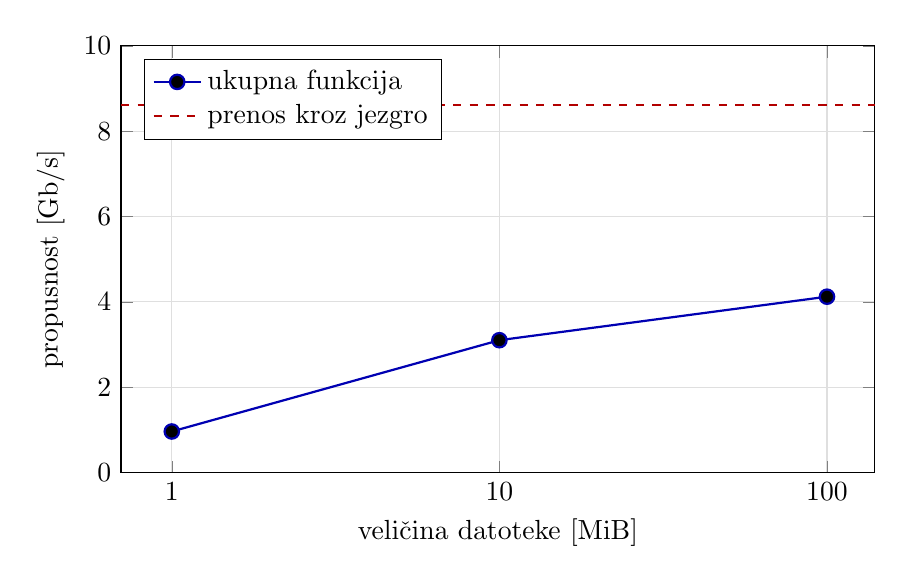
\begin{tikzpicture}
\begin{axis}[width=0.92\textwidth, height=7cm,
    xlabel={veličina datoteke [MiB]}, ylabel={propusnost [Gb/s]},
    xmode=log, log basis x=10, xtick={1,10,100}, xticklabels={1,10,100},
    xmin=0.7, xmax=140, ymin=0, ymax=10,
    grid=major, grid style={gray!25},
    legend pos=north west, legend cell align=left,
    every axis plot/.append style={thick, mark size=2.6pt}]
\addplot[mark=*, draw=blue!70!black] coordinates {(1,0.96) (10,3.10) (100,4.12)};
\addlegendentry{ukupna funkcija}
\addplot[draw=red!70!black, dashed, no marks] coordinates {(0.7,8.62) (140,8.62)};
\addlegendentry{prenos kroz jezgro}
\end{axis}
\end{tikzpicture}
\caption{Propusnost u zavisnosti od veličine datoteke}
\label{fig:sha3_rezija}
\end{figure}

\section{AES-GCM akcelerator}
\label{sec:rez_aes}

\subsection{Provera po nivoima}
\label{subsec:rez_aes_provera}

Ispravnost je proverena testovima sa poznatim odgovorima po \cite{sp80038d}, nad celim akceleratorom. Vektori pokrivaju pakete sa pridruženim podacima, nepotpun poslednji blok i dešifrovanje sa proverom oznake. Ispravnost razmene preko AXI4-Stream interfejsa proverena je i pod zastojima na oba kraja toka. Regresija broji 36 testova nad jezgrom i omotačima, među njima i promenu ključa usred paketa, a nad celim lancem još 209 slučajeva u četiri skupa, od poznatih odgovora sa prolazom po dužinama do petlje šifrovanje-dešifrovanje. Pun IPsec par uz to prolazi 120 od 120 krugova, u kojima se paket šifruje, dešifruje i vraća bajt-identičan. Serije teku pod GHDL-om, a testovi sa spoljnim imenima signala i merenja celog puta pod Vivado simulatorom.
\smallbreak
Akcelerator je proveren i u postojećem mrežnom sistemu, u kome instrument MTS 5800 služi kao generator saobraćaja, a paketi prolaze kroz sistemski omotač na vezi od 10 Gb/s. Veza je sporija od jezgra, pa propusnost ograničava ona, a ne akcelerator. Svrha te provere nije brojka nego verodostojnost, jer jezgro šifruje saobraćaj kakav na mreži zaista postoji, sa paketima promenljivih dužina i razmaka.

\subsection{Zauzeće resursa i radna učestanost}
\label{subsec:rez_aes_resursi}

Merenja idu po tri nivoa. Najpre samo AES jezgro, zatim GHASH jedinica i GCM sloj koji je vezuje za jezgro, a ceo put podataka sa sistemskim omotačem meri se u odeljku \ref{subsec:rez_aes_ceo_put}. AES jezgro implementirano je u šesnaest konfiguracija, koje pokrivaju obe arhitekture, obe realizacije runde i oba stila upravljanja tokom, a kod višejezgarne i šest brojeva jezgara. Uz njih su implementirane GHASH jedinica i GCM sloj, u obe vremenske organizacije. Rezultati su dati u tabelama \ref{tab:aes_impl_unrolled}, \ref{tab:aes_impl_multi} i \ref{tab:ghash_impl}. Propusnost je izvedena po jednačini \eqref{eq:metod_propusnost}, iz modelskih bita po taktu samog jezgra, koji za protočnu arhitekturu iznose 128, a za višejezgarnu $128 \cdot \texttt{NUM\_CORES}/(N_r+1)$ po jednačini \eqref{eq:multicore_propusnost}, a merenja iz odeljka \ref{subsec:rez_aes_propusnost} ih potvrđuju unutar procenta.

\begin{table}[H]
\caption{Protočna arhitektura, implementacija van konteksta}
\centering
{\renewcommand{\arraystretch}{1.25}
\resizebox{0.9\textwidth}{!}{
\begin{tabular}{|c|c|c|c|c|c|c|}
\hline
\rowcolor{gray!30}
Realizacija runde & Upravljanje tokom & LUT & FF & BRAM & $F_{max}$ [MHz] & Gb/s \\
\hline
\multirow{2}{*}{BRAM varijanta (T-tabele)} & \texttt{GLOBAL}     & 3339  & 5321 & 52 & 297,97 & 38,14 \\
                                          & \texttt{PER\_STAGE} & 3457  & 5414 & 52 & 299,04 & 38,28 \\
\hline
\multirow{2}{*}{LUT varijanta}                      & \texttt{GLOBAL}     & 10491 & 5320 & 0  & 401,12 & 51,34 \\
                                          & \texttt{PER\_STAGE} & 10579 & 5413 & 0  & 406,50 & 52,03 \\
\hline
\end{tabular}
}}
\label{tab:aes_impl_unrolled}
\end{table}

\begin{table}[H]
\caption{Višejezgarna arhitektura, implementacija van konteksta}
\centering
{\renewcommand{\arraystretch}{1.25}
\resizebox{0.9\textwidth}{!}{
\begin{tabular}{|c|c|c|c|c|c|c|}
\hline
\rowcolor{gray!30}
Realizacija runde & Jezgara & LUT & FF & BRAM & $F_{max}$ [MHz] & Gb/s \\
\hline
\multirow{6}{*}{BRAM varijanta (T-tabele)} & 1  & 1925  & 1843 & 4  & 307,03 & 2,62 \\
                                          & 2  & 2955  & 2239 & 8  & 314,56 & 5,37 \\
                                          & 4  & 4994  & 3024 & 16 & 288,85 & 9,86 \\
                                          & 7  & 8077  & 4204 & 28 & 282,97 & 16,90 \\
                                          & 14 & 15358 & 6960 & 56 & 278,47 & 33,27 \\
                                          & 15 & 16365 & 7355 & 60 & 263,92 & 33,78 \\
\hline
\multirow{6}{*}{LUT varijanta}                      & 1  & 2274  & 1843 & 0  & 388,80 & 3,32 \\
                                          & 2  & 3618  & 2239 & 0  & 373,12 & 6,37 \\
                                          & 4  & 5216  & 3024 & 0  & 365,10 & 12,46 \\
                                          & 7  & 8345  & 4205 & 0  & 339,44 & 20,28 \\
                                          & 14 & 15899 & 6960 & 0  & 296,12 & 35,38 \\
                                          & 15 & 16960 & 7356 & 0  & 301,93 & 38,65 \\
\hline
\end{tabular}
}}
\label{tab:aes_impl_multi}
\end{table}

Realizacija runde je kompromis između logike, memorijskih blokova i učestanosti. Protočna arhitektura u BRAM varijanti troši 3339 LUT-ova i 52 memorijska bloka na 298 MHz, a u LUT varijanti 10491 LUT, tri puta više, ali bez ijednog memorijskog bloka i na 401 MHz. Blok memorija dakle štedi logiku, a košta četvrtinu učestanosti, jer je čitanje iz memorije sporije od plitke kombinacione mreže. Kod višejezgarne arhitekture dve realizacije završavaju na skoro istom broju LUT-ova, a razlog je dat u odeljku \ref{subsec:rez_aes_arhitekture}. Poređenje stilova upravljanja tokom dato je u odeljku \ref{subsec:rez_aes_protivpritisak}.

\begin{table}[H]
\caption{GHASH jedinica i GCM sloj, implementacija van konteksta}
\centering
{\renewcommand{\arraystretch}{1.25}
\resizebox{0.9\textwidth}{!}{
\begin{tabular}{|c|c|c|c|c|c|}
\hline
\rowcolor{gray!30}
Modul & \texttt{MULT\_CYCLES} & LUT & FF & $F_{max}$ [MHz] & granica [Gb/s] \\
\hline
\multirow{2}{*}{GHASH jedinica} & 1 & 4707 & 390  & 262,86 & 33,65 \\
                                & 2 & 4382 & 960  & 348,51 & 22,30 \\
\hline
\multirow{2}{*}{GCM sloj}       & 1 & 5197 & 1023 & 227,46 & 29,12 \\
                                & 2 & 5114 & 1593 & 302,18 & 19,34 \\
\hline
\end{tabular}
}}
\label{tab:ghash_impl}
\end{table}

GHASH jedinica u dvotaktnoj organizaciji skraćuje kritičnu putanju za četvrtinu, sa 3,80 na 2,87 ns, a isto važi i za ceo GCM sloj, sa 4,40 na 3,31 ns. Cena je registarska banka koja preseca množačku mrežu, oko 570 flipflopova više. Granica u bitima po taktu se prepolovljava po konstrukciji, ali granica u apsolutnim jedinicama pada samo na dve trećine, sa 33,65 na 22,30 Gb/s, jer dvotaktna organizacija radi na trećinu višoj učestanosti. Šta ta organizacija znači na celom putu podataka, dato je u odeljku \ref{subsec:rez_aes_ceo_put}.

\subsection{Poređenje protočne i višejezgarne arhitekture}
\label{subsec:rez_aes_arhitekture}

Obe arhitekture dostižu blok po taktu, pa se razlika svodi na cenu kojom se do njega stiže. Poređenje se i ovde odnosi na samo AES jezgro, bez autentifikacionog puta. Protočna arhitektura u BRAM varijanti taj protok drži sa 3339 LUT-ova. Višejezgarnoj je za isti protok potrebno petnaest jezgara, jer svako jezgro drži blok $N_r + 1 = 15$ taktova, pa u istoj varijanti troši 16365 LUT-ova, 4,9 puta više. Kada se propusnost svede na utrošenu logiku, protočna arhitektura daje pet i po puta više megabita u sekundi po jednom LUT-u u BRAM varijanti, a dvostruko više u LUT varijanti. Zauzeće višejezgarne pritom raste gotovo linearno, od jednog do petnaest jezgara za oko 1030 LUT-ova po jezgru u BRAM i oko 1050 u LUT varijanti. Svako jezgro uz logiku runde nosi i sopstveni raspored ključeva u distribuiranoj memoriji (odeljak \ref{subsec:hw_aes_kljuc}), koji se u zauzeću vidi kao 74 LUT-a po jezgru, manje od desetine cene jezgra.
\smallbreak
Kod višejezgarne arhitekture dve realizacije runde završavaju skoro izjednačene po zauzeću, iako T-tabele u blok memoriji i ovde štede logiku glavnih rundi. Uštedu poništava završna runda, koja u BRAM varijanti u svakom jezgru nosi zaseban sloj od šesnaest S-boksova, dok u LUT varijanti prolazi bez sopstvenog (odeljak \ref{subsec:hw_aes_round_style}). Na petnaest jezgara BRAM varijanta zato staje u svega šest stotina LUT-ova manje, a za to plaća 60 memorijskih blokova i za oko 40 MHz nižu učestanost. Za višejezgarnu arhitekturu je LUT varijanta prirodan izbor.
\smallbreak
Prednost višejezgarne organizacije je granulacija. Broj jezgara je generik, pa se propusnost bira pri sintezi i plaća srazmerno cilju, dok protočna arhitektura postoji samo kao cela. Na dnu opsega jedno jezgro u BRAM varijanti staje u 1925 LUT-ova i četiri memorijska bloka, a LUT varijanta za 349 LUT-ova više izbegava i ta četiri bloka. Protočna arhitektura i tada traži ceo niz od 10491 LUT ili 52 bloka, uz 5320 flipflopova naspram 1843 koliko nosi jedno jezgro. Svako jezgro donosi petnaestinu punog protoka po ceni od oko 1050 LUT-ova, pa je za ciljeve do 20,28 Gb/s, dokle stiže sedam jezgara, višejezgarna arhitektura jeftinija od cele protočne po oba zauzeća, 8345 naspram 10491 LUT i 4205 naspram 5320 flipflopova. Iznad te granice svaka naredna konfiguracija dostiže zauzeće uporedivo sa protočnim ili veće, a protok joj ostaje manji, pa protočna arhitektura postaje sve efikasnija. Na četrnaest jezgara višejezgarna arhitektura troši 15899 LUT-ova, oko 50 procenata više od protočne, a dostiže 35,38 Gb/s, dok protočna sa 10491 LUT daje 51,34 Gb/s. Sve konfiguracije prikazane su na slici \ref{fig:aes_lut_gbps}.

\begin{figure}[H]
\centering
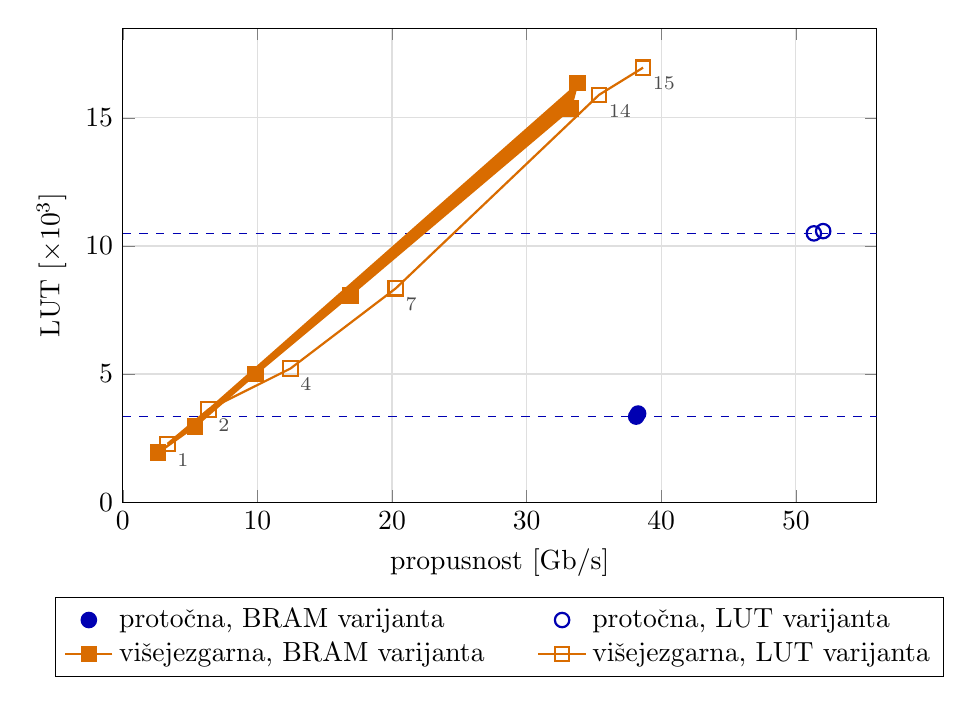
\begin{tikzpicture}
\begin{axis}[width=0.92\textwidth, height=7.6cm,
    xlabel={propusnost [Gb/s]}, ylabel={LUT [$\times 10^3$]},
    xmin=0, xmax=56, ymin=0, ymax=18.5,
    grid=major, grid style={gray!25},
    legend style={at={(0.5,-0.20)}, anchor=north, legend columns=2,
        /tikz/every even column/.append style={column sep=0.6cm}},
    legend cell align=left,
    every axis plot/.append style={thick, mark size=2.6pt}]
\addplot[draw=blue!70!black, dashed, thin, mark=none, forget plot] coordinates
    {(0,3.339) (56,3.339)};
\addplot[draw=blue!70!black, dashed, thin, mark=none, forget plot] coordinates
    {(0,10.491) (56,10.491)};
\addplot[only marks, mark=*, draw=blue!70!black, fill=blue!70!black] coordinates
    {(38.14,3.339) (38.28,3.457)};
\addlegendentry{protočna, BRAM varijanta}
\addplot[only marks, mark=o, draw=blue!70!black] coordinates
    {(51.34,10.491) (52.03,10.579)};
\addlegendentry{protočna, LUT varijanta}
\addplot[mark=square*, draw=orange!85!black, fill=orange!85!black] coordinates
    {(2.62,1.925) (5.37,2.955) (9.86,4.994) (16.90,8.077) (33.27,15.358) (33.78,16.365)};
\addlegendentry{višejezgarna, BRAM varijanta}
\addplot[mark=square, draw=orange!85!black] coordinates
    {(3.32,2.274) (6.37,3.618) (12.46,5.216) (20.28,8.345) (35.38,15.899) (38.65,16.960)};
\addlegendentry{višejezgarna, LUT varijanta}
\node[font=\scriptsize, color=gray!60!black, anchor=north west] at (axis cs:3.32,2.274) {1};
\node[font=\scriptsize, color=gray!60!black, anchor=north west] at (axis cs:6.37,3.618) {2};
\node[font=\scriptsize, color=gray!60!black, anchor=north west] at (axis cs:12.46,5.216) {4};
\node[font=\scriptsize, color=gray!60!black, anchor=north west] at (axis cs:20.28,8.345) {7};
\node[font=\scriptsize, color=gray!60!black, anchor=north west] at (axis cs:35.38,15.899) {14};
\node[font=\scriptsize, color=gray!60!black, anchor=north west] at (axis cs:38.65,16.960) {15};
\end{axis}
\end{tikzpicture}
\caption{Zauzeće i propusnost svih šesnaest AES konfiguracija. Brojevi uz tačke višejezgarne LUT varijante su broj jezgara, isprekidane linije su nivoi zauzeća protočne arhitekture}
\label{fig:aes_lut_gbps}
\end{figure}

\subsection{Propusnost u ustaljenom stanju}
\label{subsec:rez_aes_propusnost}

Propusnost je merena istim postupkom kao kod SHA-3 jezgra, takt-tačno u simulaciji, nad porukom od 512 reči širine 128 bitova, bez pridruženih podataka, dakle nad osam kilobajta korisnog sadržaja, uz ulaz koji uvek ima spremnu reč i izlaz uvek spreman da je primi. Prozor merenja počinje prvom prihvaćenom ulaznom rečju, a zatvara se izlaznom rečju oznake. Ključ i nonce zadaju se pre prve reči, pa priprema potključa $H$ i početak brojačkog niza ostaju ispred prozora. Meri se dakle ustaljeno stanje, a ne latencija prvog bloka. Oznaka tako ulazi u izmereno vreme, ali ne i u brojilac, jer se broj bitova obrađenih u taktu računa nad korisnim sadržajem, pa poruka od 512 reči obrađena kroz 516 taktova daje 127,01. Na putu dešifrovanja je obrnuto, oznaka stiže sa ulazom, pa je izlaz za reč kraći. Izmerene vrednosti i model uporedo daje tabela \ref{tab:aes_bpc}.

\begin{table}[H]
\caption{Izmerena propusnost puta šifrovanja u ustaljenom stanju, uz jednotaktnu GHASH jedinicu. Ulaz je poruka od 512 reči po 128 bitova, jezgro se meri bez sistemskog omotača}
\centering
{\renewcommand{\arraystretch}{1.25}\setlength{\tabcolsep}{10pt}
\begin{tabular}{|l|c|c|c|}
\hline
\rowcolor{gray!30}
Konfiguracija & Taktova & Bita po taktu & Model \\
\hline
Protočna                & 516  & 127,01 & 128,00 \\
\hline
Višejezgarna, 1 jezgro   & 7670 & 8,54   & 8,53 \\
\hline
Višejezgarna, 2 jezgra   & 3831 & 17,11  & 17,07 \\
\hline
Višejezgarna, 4 jezgra   & 1923 & 34,08  & 34,13 \\
\hline
Višejezgarna, 7 jezgara  & 1100 & 59,58  & 59,73 \\
\hline
Višejezgarna, 8 jezgara  & 963  & 68,05  & 68,27 \\
\hline
Višejezgarna, 14 jezgara & 552  & 118,72 & 119,47 \\
\hline
Višejezgarna, 15 jezgara & 516  & 127,01 & 128,00 \\
\hline
\end{tabular}
}
\label{tab:aes_bpc}
\end{table}

Granicu propusnosti akceleratora određuju tri nezavisna ograničenja, od kojih je merodavno najmanje:
\begin{equation}
    \label{eq:aes_model}
    B \approx 128 \cdot \min\!\left(B_{\text{šifra}},\ \frac{1}{\texttt{MULT\_CYCLES}},\ 1\right) \ \text{bita po taktu},
\end{equation}
gde je $B_{\text{šifra}}$ jednako jedinici za protočnu arhitekturu, odnosno $\texttt{NUM\_CORES}/(N_r+1)$ za višejezgarnu, kao prvi član minimuma iz jednačine \eqref{eq:multicore_propusnost}. Drugi član je autentifikacioni put, a treći jedan izlazni port. Odstupanje izmerenih vrednosti od modela nigde ne prelazi jedan procenat. Kod jednog i dva jezgra izmerena vrednost je za delić procenta i iznad modela. Model je asimptotski, a brojački blokovi ne zavise od podataka, pa raspodela prvo jezgro pokrene i pre prve prihvaćene reči (odeljak \ref{subsec:hw_aes_arh}). Glava obrade tako ostane ispred prozora merenja, koji za 512 blokova broji 7670 taktova umesto modelskih $512 \cdot 15 = 7680$. Poreklo odstupanja vidi se na protočnom redu tabele. Izmerenih 516 taktova čine 512 taktova prijema i rep od četiri takta, u kome se obave poslednje množenje u GHASH jedinici, množenje nad blokom dužina i predaja reči oznake. Rep je toliko kratak zato što AES u CTR režimu šifruje brojačke blokove, koji ne zavise od podataka, pa niz za šifrovanje teče ispred poruke i poslednja reč korisnog sadržaja ne čeka ništa osim završnih koraka autentifikacije.

Model se najbolje vidi na slici \ref{fig:aes_propusnost}. Šifarski put raste linearno sa brojem jezgara sve dok ne naiđe na granicu koju postavlja GHASH jedinica, a preko toga dodavanje jezgara ne donosi ništa.

\begin{figure}[H]
\centering
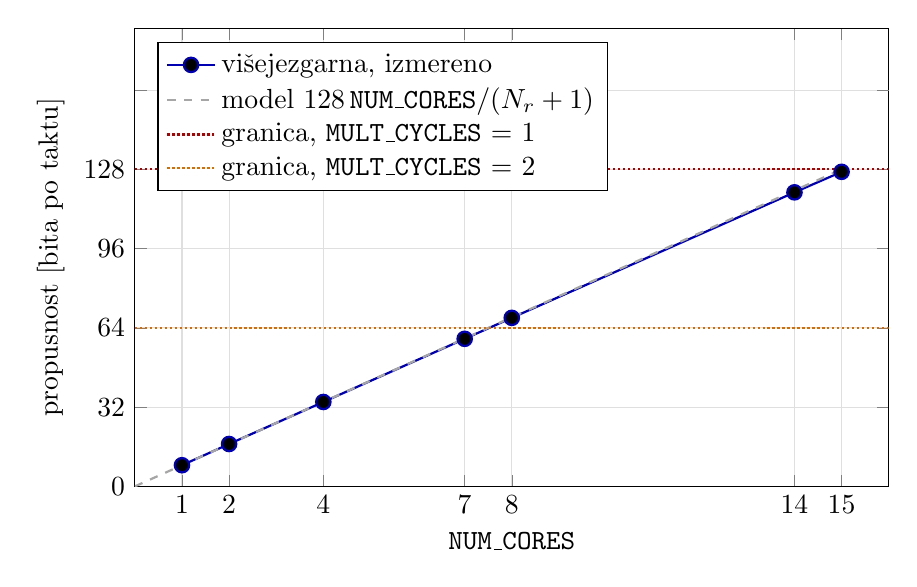
\begin{tikzpicture}
\begin{axis}[width=0.92\textwidth, height=7.4cm,
    xlabel={\texttt{NUM\_CORES}}, ylabel={propusnost [bita po taktu]},
    xtick={1,2,4,7,8,14,15}, xmin=0, xmax=16, ymin=0, ymax=185,
    ytick={0,32,64,96,128}, extra y ticks={160}, extra y tick labels={},
    grid=major, grid style={gray!25},
    legend pos=north west, legend cell align=left,
    every axis plot/.append style={thick, mark size=2.6pt}]
\addplot[mark=*, draw=blue!70!black] coordinates
    {(1,8.54) (2,17.11) (4,34.08) (7,59.58) (8,68.05) (14,118.72) (15,127.01)};
\addlegendentry{višejezgarna, izmereno}
\addplot[draw=gray!70, dashed, mark=none] coordinates {(0,0) (15,128)};
\addlegendentry{model $128\,\texttt{NUM\_CORES}/(N_r+1)$}
\addplot[draw=red!70!black, densely dotted, mark=none] coordinates {(0,128) (16,128)};
\addlegendentry{granica, \texttt{MULT\_CYCLES} = 1}
\addplot[draw=orange!85!black, densely dotted, mark=none] coordinates {(0,64) (16,64)};
\addlegendentry{granica, \texttt{MULT\_CYCLES} = 2}
\end{axis}
\end{tikzpicture}
\caption{Propusnost višejezgarne arhitekture u zavisnosti od broja jezgara}
\label{fig:aes_propusnost}
\end{figure}

Da je granica zaista na autentifikacionom putu, a ne na šifarskom, pokazuje tabela \ref{tab:aes_ghash_mera}, koja isto opterećenje propušta kroz obe vremenske organizacije GHASH jedinice iz tabele \ref{tab:ghash_granica}.

\begin{table}[H]
\caption{Propusnost pri obe vremenske organizacije GHASH jedinice}
\centering
{\renewcommand{\arraystretch}{1.25}\setlength{\tabcolsep}{10pt}
\begin{tabular}{|l|c|c|}
\hline
\rowcolor{gray!30}
Konfiguracija & \texttt{MULT\_CYCLES} = 1 & \texttt{MULT\_CYCLES} = 2 \\
\hline
Protočna                & 127,01 & 63,69 \\
\hline
Višejezgarna, 15 jezgara & 127,01 & 63,69 \\
\hline
Višejezgarna, 8 jezgara  & 68,05  & 63,69 \\
\hline
\end{tabular}
}
\label{tab:aes_ghash_mera}
\end{table}

Iz gornje tabele slede tri zaključka. Prvo, dvotaktni množač prepolovljava granicu u bitima po taktu, tačno kako model granice predviđa, i to bez obzira na broj šifarskih jezgara iza njega. To nije samo gubitak. Kraća kombinaciona putanja postiže viši takt, 302,18 naspram 227,46 MHz na GCM sloju po tabeli \ref{tab:ghash_impl}, pa je dvotaktna organizacija prirodan izbor kada cilj propusnosti staje ispod prepolovljene granice, jer se isti cilj tada postiže uz blaže vremenske uslove i sa manje jezgara. Drugo, petnaest iterativnih jezgara daje istu vrednost kao protočna arhitektura, u takt, čime se potvrđuje da su dve arhitekture zamenljive po propusnosti u taktu. U bitima u sekundi zamenljive nisu, jer višejezgarna ne dostiže učestanost protočne, kako je ranije izmereno. Treće, osam jezgara je pri dvotaktnoj jedinici dovoljno, jer njihovih $68{,}05$ bita po taktu premašuje granicu od $63{,}69$, pa se razlika ne vidi. Konfiguracije se zato biraju u paru sa vremenskom organizacijom GHASH jedinice, a ne nezavisno od nje.

\subsection{Poređenje stilova upravljanja tokom}
\label{subsec:rez_aes_protivpritisak}

Implementacija je pokazala da upravljanje tokom po stepenima (\texttt{PER\_STAGE}) košta više logike od zajedničkog (\texttt{GLOBAL}), a radnu učestanost ne menja merljivo. Ostalo je pitanje da li tu cenu opravdava ponašanje pod zastojem, koje sinteza ne može da izmeri. Zato je isto opterećenje propušteno kroz deset obrazaca zastoja. U prvoj grupi izlazna strana prima reč sa zadatom verovatnoćom po taktu, od 90 do 25 procenata. U drugoj se tako prigušuju oba kraja toka. U trećoj izlazna strana naizmenično prima zadati broj taktova pa zadati broj taktova stoji, sve do zastoja dužih od celog protočnog niza.

Nijedan obrazac ne razdvaja dva stila upravljanja, i to ne približno nego u takt. Naizmenični obrasci su uvedeni baš zato što nasumično prigušivanje po taktu nikada ne napravi dovoljno dug zastoj da se razlika pokaže, ali je ne pokazuju ni oni, uključujući zastoje od šesnaest uzastopnih taktova, koliko protočni niz ima slobodnih mesta, i dvostruko duže od toga.

Objašnjenje je u samoj protočnoj arhitekturi. Njeno dopuštenje takta uslovljeno je time da je ili izlaz spreman, ili protok još nije pun, pa glava protoka nastavlja da prima podatke i za vreme zastoja na izlazu, sve dok se ne popuni. Zajedničko upravljanje tokom tako bez dodatne logike obavlja glavni deo posla zbog kojeg je stil po stepenima uveden, punjenje niza za vreme zastoja na izlazu. Ostaje mu nedostupno jedino sabijanje mehura unutar niza, a nijedno merenje tu razliku ne pokazuje, pa je zajedničko upravljanje podrazumevani izbor.

Propusnost pritom verno prati raspoloživost izlaza. Kada izlaz prima polovinu taktova, dobija se polovina pune vrednosti, kada prima četvrtinu, četvrtina, a kada prima tri četvrtine taktova, tri četvrtine pune vrednosti. Akcelerator ni u jednom obrascu nije usko grlo, nego propušta onoliko koliko mu okolina dozvoli.

\subsection{Mrežni paketi}
\label{subsec:rez_aes_kratki}

Vrednosti iz ustaljenog stanja važe za duge poruke, a paketi na mreži su kratki. Svaki od njih nosi režiju. Novi nonce menja ceo brojački niz, pa se na granici paketa zatečeni višak starog niza obriše u jednom taktu, ali protočni niz time ostane prazan, i prva reč novog paketa čeka da novi blok $J_0$ i prvi brojački blok prođu kroz ceo niz, dok izlaz pre toga nosi još reč oznake prethodnog paketa. Potključ $H$ u toj režiji ne učestvuje, jer zavisi samo od ključa, pa ga omotač čuva dok se ključ ne promeni. Zato je ista serija ponovljena nad paketima mrežnih veličina, sa ukupnim količinama od četiri do dvanaest kilobajta. Rezultati su u tabeli \ref{tab:aes_kratki}.

\begin{table}[H]
\caption{Propusnost pri mrežnim veličinama paketa, protočna arhitektura}
\centering
{\renewcommand{\arraystretch}{1.25}\setlength{\tabcolsep}{10pt}
\begin{tabular}{|c|c|c|c|c|}
\hline
\rowcolor{gray!30}
Paket & Reči & Paketa & Bita po taktu & Udeo granice \\
\hline
64 B    & 4   & 64 & 22,49  & 17,7 \% \\
\hline
512 B   & 32  & 16 & 81,82  & 64,4 \% \\
\hline
1504 B  & 94  & 8  & 108,27 & 85,2 \% \\
\hline
duga poruka & 512 & 1 & 127,01 & 100 \% \\
\hline
\end{tabular}
}
\label{tab:aes_kratki}
\end{table}

Sve redove sa više paketa objašnjava jedna veličina, režija po paketu od oko osamnaest taktova. Ona se čita neposredno iz merenja. Šezdeset četiri paketa od po četiri reči obrađena su kroz 1457 taktova, višak od 18,8 taktova po paketu, a osam paketa od po 94 reči kroz 889 taktova, višak od 17,1. Za pakete od 1504 bajta taj višak znači 85 procenata pune vrednosti, pa realan saobraćaj radi blizu granice akceleratora. Kod paketa od 64 bajta režija nadjača koristan rad od svega četiri reči i propusnost padne na nepunu petinu. Šta od ove režije ostane na celom putu podataka, pokazuje odeljak \ref{subsec:rez_aes_ceo_put}.

Praktična posledica je da se puna vrednost akceleratora dobija na dugim paketima. Pri najkraćim paketima merodavna je režija po paketu, a ona potiče od samog režima rada, jer svaki novi nonce traži nov brojački niz.

\subsection{Ceo put podataka}
\label{subsec:rez_aes_ceo_put}

Dosadašnja merenja obuhvatala su AES jezgro, GHASH jedinicu i GCM sloj svaki za sebe. Ostaje ono što bi se u sistem zaista ugradilo, ceo put podataka zajedno sa sistemskim omotačem iz odeljka \ref{subsec:hw_l3}, i to u oba smera. Zaglavlje je dimenzionisano po ESP-u u tunelskom režimu preko Etherneta i IPv4, pa se 34 bajta prenose nepromenjena, a 16 bajtova ESP zaglavlja i eksplicitnog inicijalizacionog vektora ulazi u pridružene podatke. Zauzeće, učestanost i propusnost oba smera daje tabela \ref{tab:aes_ceo_put}.

\begin{table}[H]
\caption{Ceo put podataka nad paketima ESP tunela. Red \textit{GCM lanac} je GCM sloj sa AES jezgrom, red \textit{sa omotačem} isti lanac uz razdvajanje, sastavljanje i poravnanje oznake. Obe arhitekture su u LUT varijanti, a GHASH jedinica je jednotaktna}
\centering
{\renewcommand{\arraystretch}{1.25}
\resizebox{\textwidth}{!}{
\begin{tabular}{|c|c|c|c|c|c|c|c|}
\hline
\rowcolor{gray!30}
\multicolumn{2}{|c|}{} & \multicolumn{3}{c|}{višejezgarna, 15 jezgara} & \multicolumn{3}{c|}{protočna} \\
\cline{3-8}
\rowcolor{gray!30}
Nivo & Smer & LUT & $F_{max}$ [MHz] & Gb/s & LUT & $F_{max}$ [MHz] & Gb/s \\
\hline
\multirow{2}{*}{GCM lanac}   & šifrovanje   & 21908 & 223,14 & 28,56 & 15510 & 224,27 & 28,71 \\
                             & dešifrovanje & 22210 & 221,02 & 28,29 & 15613 & 228,42 & 29,24 \\
\hline
\multirow{2}{*}{sa omotačem} & šifrovanje   & 23518 & 228,65 & 29,27 & 16765 & 239,82 & 30,70 \\
                             & dešifrovanje & 25015 & 218,18 & 27,93 & 18729 & 230,64 & 29,52 \\
\hline
\end{tabular}
}}
\label{tab:aes_ceo_put}
\end{table}

Protočna arhitektura zadržava prednost i na celom putu podataka. Logike joj treba od 1,34 do 1,42 puta manje. Razlike u učestanosti, od 0,5 do 5,7 procenata u njenu korist, ostaju unutar šuma alata iz odeljka \ref{sec:rez_metodologija}, pa se sme tvrditi samo da protočna arhitektura manju površinu ne plaća učestanošću.
\smallbreak
Sistemski omotač košta od 1255 do 3116 LUT-ova, više na putu dešifrovanja, jer uz razdvajanje i sastavljanje tamo stoji i poravnanje oznake. Učestanost se pritom menja u granicama šuma, a na putu šifrovanja protočne arhitekture omotač je čak podiže, sa 224,27 na 239,82 MHz, jer skid baferi omotača (odeljak \ref{subsec:hw_axis}) seku putanje koje bi inače prelazile granicu jezgra.
\smallbreak
Granicu učestanosti celog puta podataka postavlja GCM sloj. Od delova koji se mere zasebno GHASH jedinica postiže 262,86 MHz, GCM sloj 227,46, a AES blok 301,93 u višejezgarnoj i 401,12 u protočnoj varijanti, prema tabelama \ref{tab:ghash_impl}, \ref{tab:aes_impl_multi} i \ref{tab:aes_impl_unrolled}. Najniža je vrednost GCM sloja i svih osam merenja staje u njenoj okolini, od 218 do 240 MHz, u granicama šuma alata. AES blok granici ne prilazi ni u jednoj varijanti, pa se izbor arhitekture na učestanost celog puta ne odražava. Put podataka pritom daje blok po taktu, 128 bita po taktu, pa je gornja granica propusnosti sistema oko 30 Gb/s, a najviše izmereno 30,70.
\smallbreak
Propusnost ispod te granice bira se brojem jezgara, po jednačini \eqref{eq:aes_model}. Za cilj od 10 Gb/s dovoljno je šest jezgara, jer šest petnaestina granice GCM sloja od 29,12 Gb/s iznosi 11,6, dok pet daje 9,7. Najbliža merena konfiguracija, sedam jezgara sa 8345 LUT-ova u jezgru, cilj pokriva sa rezervom, za manje od polovine logike punih petnaest. Granica isplativosti višejezgarne varijante iz odeljka \ref{subsec:rez_aes_arhitekture} važi i sa omotačem, jer GCM sloj i omotač koštaju približno isto u obe varijante, na putu šifrovanja 6558 naspram 6274 LUT-ova preko golog jezgra, a na putu dešifrovanja 8055 naspram 8238, pa se poređenje i ovde svodi na samo jezgro. U propusnosti ta granica na celom putu znači manje nego na golom jezgru. Sedam jezgara ovde nosi sedam petnaestina granice GCM sloja, oko 13,6 Gb/s, jer ceo put radi na učestanosti sloja, a ne jezgra. Dupleksni par sa omotačem, šifrovanje i dešifrovanje zajedno, staje u 48533 LUT-a u višejezgarnoj varijanti, odnosno 41,4 procenta čipa, a u protočnoj u 35494 LUT-a, odnosno 30,3 procenta.
\smallbreak
Dvotaktna GHASH jedinica pomera granicu učestanosti celog puta podataka na oko 260 MHz. Sa njom GCM sloj sam postiže 302,18 MHz, a AES blok 301,93, ali deo te razlike ode na cenu spajanja, pa GCM lanac dostiže 266,18, a put sa omotačem 258,76 MHz. Granica u bitima po taktu se pritom prepolovi, pa propusnost padne sa oko 30 na oko 17 Gb/s, 64 bita po taktu na izmerenoj učestanosti, i jednotaktna organizacija ostaje radna tačka za najveću propusnost. Kada dvotaktna ipak ima smisla, pokazano je u odeljku \ref{subsec:rez_aes_propusnost}.
\smallbreak
Uz zauzeće i učestanost izmerena je, takt-tačno u simulaciji, i propusnost celog puta sa omotačem, nad nizom paketa sa korisnim sadržajem od 1504 bajta u istom rasporedu segmenata. Rezultat je dat u tabeli \ref{tab:aes_put_propusnost}. Od 111 taktova po paketu 99 nosi reči paketa. Zastoj od dvanaest taktova čine osam taktova punjenja jezgra novim brojačkim nizom, tri takta čekanja na reč oznake i jedan takt na preklopu segmenata. Samo punjenje traje koliko i protočni niz, ali mu se početak sakrije ispod reči oznake i segmenata koji kroz jezgro ne prolaze, pa se vidi samo osam taktova. Vrednost je ista za obe arhitekture, jer obe drže blok po taktu pa je tok reči kroz put podataka identičan. Poklapanje sa vrednošću izmerenom bez omotača pokazuje da sistemski omotač ne košta propusnost. Istim nizom paketa proveren je i pun krug, u kome se svaki paket šifruje kroz šifarski IP, dešifruje kroz IP za dešifrovanje i vraća bajt-identičan uz potvrđenu oznaku.

\begin{table}[H]
\caption{Propusnost celog puta podataka u ustaljenom stanju, nad paketima sa korisnim sadržajem od 1504 bajta. Kolona \textit{bez omotača} je isti sadržaj iz tabele \ref{tab:aes_kratki}}
\centering
{\renewcommand{\arraystretch}{1.25}
\resizebox{0.9\textwidth}{!}{
\begin{tabular}{|c|c|c|c|c|}
\hline
\rowcolor{gray!30}
Reči po paketu & Zastoj [taktova] & Taktova po paketu & Korisni sadržaj [b/takt] & Bez omotača [b/takt] \\
\hline
99 & 12 & 111 & 108,40 & 108,27 \\
\hline
\end{tabular}
}}
\label{tab:aes_put_propusnost}
\end{table}

\section{Sistem u celini}
\label{sec:rez_sinteza}

Tri jezgra zajedno pokrivaju ceo hibridni tok iz odeljka \ref{sec:hibridni_sistem}, a merenja iz ovog poglavlja daju svakom od njih radnu tačku. ECDH jezgro je familija od petnaest izmerenih konfiguracija u kojoj se površina i trajanje biraju generikom. Paralelno jezgro na približno istoj površini daje 2,7 puta kraće skalarno množenje, a najbolji proizvod površine i vremena mu je trećinu povoljniji od osnovnog. SHA-3 jezgro u prvoj arhitekturi postiže više od 400 MHz u svih sedam konfiguracija, a dvostruko zauzeće druge arhitekture nigde ne donosi dobitak izvan šuma alata, najbliže mu prilazi SHA3-512 sa magistralom od 64 bita. Kod AES-GCM akceleratora obe arhitekture dostižu blok po taktu. Protočna do njega stiže sa manje logike, pa je izbor za najveću propusnost, sa 30,70 Gb/s na celom putu podataka, dok dupleksni par sa omotačem staje u 30 procenata čipa (odeljak \ref{subsec:rez_aes_ceo_put}). Višejezgarna se plaća po jezgru, pa je jeftinija za ciljeve do oko 20 Gb/s na nivou jezgra, odnosno do oko 13,6 Gb/s na celom putu podataka. Na paketima realnih veličina akcelerator zadržava 85 procenata pune vrednosti.

\smallbreak
Isti izbor konfiguracija daje i budžet čipa. Radna tačka ECDH jezgra, paralelna konfiguracija sa $D = 32$, zauzima 58112 LUT-ova i 25511 flipflopova, SHA-3 jezgro u prvoj arhitekturi kao SHA3-512 sa magistralom od 64 bita 4803 i 2882, a dupleksni AES-GCM par sa omotačem u protočnoj LUT varijanti 35494 i 15984. Zbir implementacija van konteksta iznosi 98409 LUT-ova, oko 84 procenta čipa, i 44377 flipflopova, ispod petine od 234240 raspoloživih. Taj zbir je procena, jer zajedničko rutiranje sva tri jezgra nije izvedeno, ali pokazuje da izabrane radne tačke na ploču staju sa oko 16 procenata rezerve u logici. Rezerva se može i proširiti, jer protočno jezgro postoji i u BRAM varijanti, koja rundu drži u blok memoriji. Dupleksni par tada po istom računu pada na oko 21 hiljadu LUT-ova uz 104 memorijska bloka od 144 raspoloživa, koje druga dva jezgra ne koriste, pa ukupan zbir silazi na oko 84 hiljade LUT-ova, oko 72 procenta čipa. Pošto je na ovoj ploči upravo logika kritičan resurs, ta zamena je povoljnija, a učestanost celog puta ne menja, jer i BRAM varijanta jezgra ostaje iznad granice GCM sloja. Svako osetnije proširenje ipak traži veću platformu (poglavlje \ref{ch:unapredjenja}).

\smallbreak
Zajednički rad sva tri jezgra proveren je simulacijom celog lanca sa slike \ref{fig:hw_lanac}, sa obe strane veze. Svaka strana ima svoje ECDH i SHA-3 jezgro i svoj par punih AES-GCM IP-ova sa sistemskim omotačem, u istom rasporedu segmenata ESP tunela kao na celom putu podataka, pa strane uspostavljaju ključ i njime razmenjuju pakete. Postavka je prikazana na slici \ref{fig:sim_lanac}. Verifikaciono okruženje igra ulogu upravljačke logike okvira, pa javne ključeve prenosi onako kako su izračunati, sklapa KMAC okvir oko tajne $Z$ po odeljku \ref{subsec:kmac} i izvedeni ključ predaje AES-GCM lancu. ECDH jezgra rade u paralelnoj konfiguraciji sa $D = 64$, izabranoj da skalarno množenje u simulaciji traje što kraće, a provera teče na Vivado simulatoru.

\begin{figure}[H]
\centering
\resizebox{0.88\textwidth}{!}{
\begin{tikzpicture}[tajna/.style={thick,->,>=stealth,red!70!black},
    okvir/.style={rectangle, rounded corners, draw=black, fill=gray!35, minimum width=3.2cm, minimum height=1.1cm, align=center}]
    % side A
    \node (ecdha) [blokkripto, minimum width=3.2cm, minimum height=1.1cm] at (0,7.0) {ECDH};
    \node (okvira) [okvir] at (0,4.7) {upravljačka\\ logika okvira};
    \node (sha3a) [blokkripto, minimum width=3.2cm, minimum height=1.1cm, align=center] at (0,2.35) {SHA-3\\ (cSHAKE)};
    \node (aesa)  [blokkripto, minimum width=3.2cm, minimum height=1.1cm, align=center] at (0,0) {AES-GCM\\ (IPsec IP)};
    % side B
    \node (ecdhb) [blokkripto, minimum width=3.2cm, minimum height=1.1cm] at (9.4,7.0) {ECDH};
    \node (okvirb) [okvir] at (9.4,4.7) {upravljačka\\ logika okvira};
    \node (sha3b) [blokkripto, minimum width=3.2cm, minimum height=1.1cm, align=center] at (9.4,2.35) {SHA-3\\ (cSHAKE)};
    \node (aesb)  [blokkripto, minimum width=3.2cm, minimum height=1.1cm, align=center] at (9.4,0) {AES-GCM\\ (IPsec IP)};
    % side labels
    \node [font=\small\itshape] at (0,7.95) {strana A};
    \node [font=\small\itshape] at (9.4,7.95) {strana B};
    % scalars
    \node (da) [font=\small] at (-3.3,7.0) {skalar $d_A$};
    \node (db) [font=\small] at (12.7,7.0) {skalar $d_B$};
    \draw [strelica] (da) -- (ecdha);
    \draw [strelica] (db) -- (ecdhb);
    % public key exchange
    \draw [strelica, <->] (ecdha) -- node[above, font=\small] {javni ključevi} (ecdhb);
    % secret material and KMAC frame
    \draw [tajna] (ecdha) -- node[right, font=\small] {tajna $Z$} (okvira);
    \draw [tajna] (ecdhb) -- node[left, font=\small] {tajna $Z$} (okvirb);
    \draw [strelica] (okvira) -- node[right, font=\small] {KMAC okvir} (sha3a);
    \draw [strelica] (okvirb) -- node[left, font=\small] {KMAC okvir} (sha3b);
    \draw [tajna] (sha3a) -- node[right, font=\small] {ključ $K$} (aesa);
    \draw [tajna] (sha3b) -- node[left, font=\small] {ključ $K$} (aesb);
    % protected packets, both directions
    \draw [strelica] ([yshift=0.28cm]aesa.east) -- node[above, font=\small] {zaštićeni paketi} ([yshift=0.28cm]aesb.west);
    \draw [strelica] ([yshift=-0.28cm]aesb.west) -- ([yshift=-0.28cm]aesa.east);
    % testbench frame
    \draw [dashed, thick, black!60] (-4.8,-1.0) rectangle (14.2,8.5);
    \node [anchor=south west, font=\small\itshape] at (-4.7,8.55) {verifikaciono okruženje};
\end{tikzpicture}
}
\caption{Lanac u simulaciji sa dve strane. Crvene strelice nose tajni materijal}
\label{fig:sim_lanac}
\end{figure}
\smallbreak
Provera prolazi kroz sve karike. Obe strane izračunaju istu tajnu $Z$, jednaku referentnom modelu. Obe iz nje izvedu isti ključ sesije od 256 bita, ponovo jednak referentnom. Paket od 64 bajta putuje od jedne strane do druge, a nazad paket od 40 bajtova sa drugom nonce vrednošću. Šifrati i oznake poklapaju se sa referentnim modelima, primalac svaki paket vraća bajt-identičan i potvrđuje oznaku. Ceo tok, od predaje skalara do poslednje potvrđene oznake, staje u 33\,290 taktova, od čega dva uzastopna skalarna množenja po strani nose gotovo sve. Time je popunjen i poslednji red tabele \ref{tab:nivoi_provere}, pa je svaki nivo, od operacije u polju do zajedničkog rada celog lanca, pokriven bar jednom nezavisnom proverom. Pravci u kojima se sistem odavde razvija razmotreni su u poglavlju \ref{ch:unapredjenja}.
